%% Mechanical Systems and Signal Processing -- Elsevier CAS double-column class (els-cas-templates on CTAN),
%% numbered references. Derived from main.tex by scripts/make_dc.py; edit main.tex, not this file.
\documentclass[a4paper,fleqn]{cas-dc}

\usepackage[numbers,sort&compress]{natbib}
\usepackage{threeparttable}
\usepackage{tikz}
\usetikzlibrary{arrows.meta,positioning,shapes.geometric,calc,decorations.pathreplacing,decorations.pathmorphing}
\newcolumntype{L}[1]{>{\raggedright\arraybackslash}p{#1}}
\newcolumntype{C}[1]{>{\centering\arraybackslash}p{#1}}
\hypersetup{colorlinks=true,linkcolor=blue!60!black,citecolor=blue!60!black,urlcolor=blue!60!black,
            pdftitle={A signal-to-drift ratio for winding-fault detectability and sensor selection in three wind-turbine generator--drive systems},
            pdfauthor={Hüseyin Tayyer Canseven}}
\usepackage{xurl}      % URLs and DOIs may break at any character (loaded after hyperref)
\urlstyle{same}
\graphicspath{{figures/}}

%% References print the DOI as a resolvable link (Elsevier style) instead of the bst's `doi:' prefix.
\providecommand{\DOIprefix}{}
\newcommand{\doi}[1]{\href{https://doi.org/#1}{\nolinkurl{https://doi.org/#1}}}

%% Float placement: allow figures and tables to share pages with text and with each other.
\renewcommand{\topfraction}{0.9}
\renewcommand{\bottomfraction}{0.7}
\renewcommand{\textfraction}{0.07}
\renewcommand{\floatpagefraction}{0.8}
\renewcommand{\dbltopfraction}{0.9}
\renewcommand{\dblfloatpagefraction}{0.8}
\setcounter{topnumber}{3}
\setcounter{dbltopnumber}{3}
\setcounter{totalnumber}{4}
%% Table body size (the class sets captions and references at 8 pt).
\newcommand{\tabsize}{\fontsize{8}{10}\selectfont}
%% Reference list at the class's 8 pt on a slightly tighter leading (the class sets 8/10 at begin-document).
\AtBeginDocument{\gdef\bibfont{\fontsize{8}{9.5}\selectfont}}
\setlength{\emergencystretch}{1.5em}
%% The class prints an `ORCID(s):' footnote even when no ORCID is given; none is given here.
\makeatletter
\AtBeginDocument{\RenewDocumentCommand\printorcid{}{}}
\makeatother

\begin{document}
\let\WriteBookmarks\relax
\shorttitle{A signal-to-drift ratio for winding-fault detectability and sensor selection}
\shortauthors{H.~T. Canseven}

\title[mode=title]{A signal-to-drift ratio for winding-fault detectability and sensor selection in three wind-turbine generator--drive systems}

\author[1]{H\"useyin Tayyer Canseven}
\ead{huseyin.canseven@lut.fi}
\credit{Conceptualization, Methodology, Software, Formal analysis, Investigation, Data curation, Visualization, Writing -- original draft, Writing -- review \& editing}
\affiliation[1]{organization={Department of Electrical Engineering, LUT School of Energy Systems, LUT University},
                city={Lappeenranta},
                postcode={53850},
                country={Finland}}

\begin{abstract}
Winding-fault detection is developed one machine at a time, so how the generator and its drive change the problem is unquantified. This paper proposes a statistic for seeded-fault campaigns that needs neither a model nor a trained detector: the signal-to-drift ratio (SDR), the change of a feature from a healthy reference interval to a faulted one, divided by a quantile of its changes between adjacent healthy intervals. The SDR is a known-onset mean-shift statistic scaled by the machine's healthy variability; its threshold needs no separate healthy campaign, though validating the false-alarm rate does. From it follow a minimum detectable extent, the extent detected with power 0.9 and a signature location per machine, suite and class; a decision table selects the cheapest adequate suite, and a transfer test fixes the feature-referencing rule of a shared detector. The method is demonstrated on open bench data of a permanent-magnet, an induction and a wound-field generator with the same tapped short-circuits. The same design-level fault is a different physical event in each machine, and phasor residuals remove a faulted-phase dependence of the negative-sequence ratios. The signature relocates between terminal voltage, controller states and field current with the machine--drive combination; the common bench's two machines differ in terminal impedance by a factor 1.7. On that bench no suite detects the smallest inter-turn level with power 0.9, the middle level is met by drive-internal quantities alone, and a learned detector transfers for abrupt-onset detection (AUC 0.85 to 0.98) once referenced to the target machine's healthy behaviour.
\end{abstract}

\begin{highlights}
\item A drift-calibrated statistic quantifies seeded-fault detectability without a model
\item Phasor residuals remove the faulted-phase dependence of negative-sequence ratios
\item Signatures relocate across voltage, controller and field current by machine and drive
\item A decision table selects the cheapest suite meeting an empirical 0.9 power target
\item Healthy referencing improves cross-system transfer in the tested machines
\end{highlights}

\begin{keywords}
condition monitoring \sep probability of detection \sep stator winding fault \sep negative sequence \sep wind-turbine generators \sep sensor selection
\end{keywords}

\maketitle

\section{Introduction}\label{sec:intro}

Stator-winding insulation faults are the archetypal incipient failure of an electrical machine. A short-circuit across a few turns has a subtle signature, and it grows into a machine-destroying fault if it is not detected \citep{RieraGuasp2015}. Electrical-subsystem failures contribute substantially to wind-turbine downtime \citep{Tavner2007}. A rich literature detects winding faults in a given machine \citep{Thomson2001, Kliman1996, Lee2003, Nandi2005, Tallam2007, Tallam2003, Cruz2004}, and almost all of it is validated on one machine. Yet the generator type of a large turbine---permanent-magnet synchronous (PMSG), squirrel-cage induction (SCIG), wound-field synchronous (WFSG) or doubly-fed induction---is chosen on cost, mass, efficiency and grid-compliance grounds \citep{Polinder2013}, and its condition monitoring is added afterwards from commercial systems \citep{Yang2010, Yang2014}. Whether the same fault is equally visible in different generator--drive systems, in which measured quantity it appears, and which sensors are therefore worth specifying has not been quantified.

Such a question needs a measure of detectability with four properties. It must be computable without a model of the machine and without a trained detector. It must be comparable across features in different units, across operating points and across machines whose healthy behaviour differs. It must connect to the quantities a monitoring specification is written in: the smallest fault to be detected, the detection power, the false-alarm rate tolerated and the sensors it costs. And it must be honest about what it needs instead of a model, namely seeded faults of known extent. The detectability notions of fault detection and isolation (FDI) theory \citep{Basseville2001, Blanke2016, Krysander2008} and the sensor-placement methods built on them \citep{Frisk2009} presuppose a model. A learned detector \citep{Lei2020} presupposes data from the very machine, and its transfer across machines is an open problem \citep{Pan2010}. The probability-of-detection (POD) methodology of non-destructive evaluation \citep{MILHDBK1823A}, the limit of detection of measurement science \citep{Currie1968} and novelty detection under environmental and operational variability in structural health monitoring \citep{Sohn2007, Farrar2013} have the first three properties. They are the family this paper builds on (Section~\ref{sec:background}).

This paper proposes the signal-to-drift ratio (SDR). It is the change of an observable feature between a healthy reference interval and a faulted interval, divided by a quantile of the changes the same feature shows between adjacent healthy intervals when nothing is wrong. The SDR is the known-onset mean-shift test of change detection \citep{Basseville1993} written as a standardised effect size. Its null is taken from the two halves of the reference interval of every trial, so the threshold needs no separate healthy campaign; independent healthy records remain necessary to validate the false-alarm rate. From it follow a \emph{minimum detectable extent} (MDE), the extent $e_{90}$ detected with power 0.9, a \emph{detectable share} and a \emph{signature location} per machine, sensor suite and fault class. A decision table selects the cheapest adequate suite, and a transfer test fixes the feature-referencing rule under which a detector built on one machine serves another. The question is made answerable by open benchmark datasets \citep{Tominaga2025pmsg, Tominaga2025scig, Tominaga2024gen}. In them a PMSG, an SCIG and a variable-speed WFSG were subjected to the same inter-turn and inter-winding short-circuits at the same tapped positions of the stator winding, the PMSG and the SCIG on one bench with one converter, one controller and one protocol.

The contributions are three. First, a framework for drift-calibrated detectability assessment and sensor selection in seeded-fault test campaigns: the SDR with its screen and its calibrated oracle, the limit-of-detection quantities evaluated on the physically distinct fault sizes of a test matrix rather than on its nominal extents, and the equivalences and differences to the established effect sizes, stated and tested on the same trials. Second, a procedure that turns these quantities into a decision table with bootstrap support and into a transfer test over referencing rules. Third, the first quantitative comparison known to the author of winding-fault detectability across three generator--drive systems, with four findings. The design-level extent and the physical severity of a fault are different axes, and the faulted phase rides on the nominal extent axis unless sequence quantities are taken as phasor residuals. The measurement group in which a fault appears depends on the machine--drive combination. The cheapest adequate suite depends on the machine \emph{and} on the requirement. A learned detector transfers once its features are referenced to healthy behaviour of the target machine.

The scope is stated at the outset. The SDR quantifies the detectability of an abrupt-onset change at a stationary operating point against a healthy reference recorded immediately before it. It is the statistic of a seeded-fault campaign, as POD is, not of a continuously operating monitor; Section~\ref{sec:res-robust} quantifies what an older reference costs. One physical machine represents each generator type, so the findings are about three generator--drive systems, not about topologies.
%% ----------------------------------------------------------------------
%% background
%% ----------------------------------------------------------------------

\section{Background and related work}\label{sec:background}

Fault detection and isolation has a mature theory of diagnosability for modelled systems. Structural analysis determines which faults are detectable and isolable from which sensor sets \citep{Blanke2016, Krysander2008}, sensor placement selects the cheapest adequate set \citep{Frisk2009}, and \citet{Basseville2001} defines detectability as a distance between the residual distributions under the healthy and the faulted hypothesis. All presuppose a trusted model. Data-driven diagnosis \citep{Lei2020} replaces the model by data from the very machine, with transfer across machines an active problem \citep{Pan2010}. Prognostics grades features by trendability \citep{Coble2013} or by separability measures such as the per-feature area under the receiver operating characteristic curve (AUC) \citep{Hanley1982}.

Three further literatures are closer to the SDR than any of these, and Table~\ref{tab:positioning} places it among them. In non-destructive evaluation, the probability of detection as a function of flaw size is estimated from seeded flaws, and a monitoring requirement is written as $a_{90/95}$, the size detected with probability 0.9 at 95\,\% confidence \citep{MILHDBK1823A}. In measurement science, the limit of detection is set by a quantile of blank measurements \citep{Currie1968}. In structural health monitoring, a novelty index is calibrated on the structure's own healthy variability across its operating envelope \citep{Sohn2007, Cross2011, Farrar2013}, and population-based methods ask when a detector transfers between similar structures \citep{Bull2021, Gardner2020, Gardner2021}. The SDR is a member of this family. For a fixed feature, $\mathrm{SDR}\ge1$ is exactly a threshold on the change statistic at the empirical healthy quantile, so any normalisation followed by the same calibrated threshold takes the same decisions. What the SDR adds is not a new rejection region. It is a null that every trial supplies from its own reference interval, so that the threshold needs no separate healthy campaign, while validating the false-alarm rate still does; a dimensionless scale on which features, operating points and machines are compared; a screen and a calibrated oracle that keep the false-alarm rate honest; and the POD quantities derived from it for sensor selection. Section~\ref{sec:res-mde} tests the equivalences on the same trials. The SDR stops at detectability, which isolation, severity estimation and prognosis presuppose.

\begin{table*}[htbp]
\fontsize{8}{10}\selectfont
\setlength{\tabcolsep}{3pt}
\centering
\caption{Detectability measures: what each needs and what it yields}\label{tab:positioning}
\begin{threeparttable}
\begin{tabular}{@{}L{4.9cm}C{1.1cm}C{1.35cm}C{1.5cm}C{1.2cm}C{1.4cm}C{0.9cm}@{}}
\toprule
Measure & Model & Trained detector & Separate healthy campaign & Seeded faults & False-alarm rate & MDE \\
\midrule
Structural detectability \citep{Blanke2016, Krysander2008} & yes & no & no & no & by design & no \\
Fault-to-noise ratio \citep{Basseville2001} & yes & no & no & no & yes & yes \\
Learned detector, AUC or TPR \citep{Lei2020} & no & yes & yes & yes & yes & no \\
Per-feature AUC, Fisher criterion \citep{Hanley1982} & no & no & usual$^{\mathrm{a}}$ & yes & no & no \\
Cohen's $d$, $d'$ & no & no & usual$^{\mathrm{a}}$ & yes & Gaussian only & no \\
POD, $a_{90/95}$ \citep{MILHDBK1823A} & no & no & no & yes & separate & yes \\
Limit of detection \citep{Currie1968} & no & no & blanks & yes & yes & yes \\
Novelty index under EOV \citep{Sohn2007, Farrar2013} & no & no & yes & no & yes & no \\
SDR with screen and oracle (this paper) & no & no & no & yes & yes & yes \\
\bottomrule
\end{tabular}
\begin{tablenotes}[flushleft]
\item Separate healthy campaign: whether the measure needs healthy records beyond the reference interval of each trial (the SDR's screen uses healthy trials where they exist, but its null does not). Seeded faults: whether faults of known extent must be realised in every candidate. False-alarm rate: whether the threshold is calibrated to a stated rate; POD treats false calls separately. MDE: whether a minimum detectable extent follows directly. EOV: environmental and operational variability.
\item[a] As usually applied; both can be formed on the within-trial drift null, as Section~\ref{sec:res-mde} does, and then differ from the SDR only in the threshold.
\end{tablenotes}
\end{threeparttable}
\end{table*}

Inter-turn short-circuits are among the most studied incipient faults in electrical machines \citep{RieraGuasp2015, Zafarani2018}. Negative-sequence methods \citep{Kliman1996, Arkan2001, Lee2003}, the extended Park's vector approach \citep{Cruz2001} and the reviews \citep{Nandi2005, Tallam2007, Henao2014} have established the signatures. A winding asymmetry produces negative-sequence components in the terminal quantities and a component at twice the fundamental frequency in the synchronous frame. Because the fault-induced negative-sequence phasor adds to the inherent asymmetry of the machine, the detection quantity is the change of that phasor rather than of its magnitude \citep{Kliman1996, Arkan2001}. Under closed-loop current control the asymmetry migrates into the voltage commands and the controller states to a degree set by the current-loop bandwidth relative to twice the electrical frequency \citep{Tallam2003, Cruz2004, Cheng2011}. In a wound-field machine the stator negative sequence induces a component at twice the electrical frequency in the field current \citep{Neti2009}, and in permanent-magnet machines with an accessible neutral the zero-sequence voltage is a sensitive indicator \citep{Urresty2012, Hang2015}. These facts have not been turned into a measure applicable across candidate machines. Learned detectors are developed for one machine \citep{Canseven2026machines}, and finite-element turn-fault models \citep{Vaseghi2009} are the natural trial generators before hardware exists.
%% ----------------------------------------------------------------------
%% method
%% ----------------------------------------------------------------------

\section{Method}\label{sec:method}

\subsection{Definitions and terms}\label{sec:defs}

Let $\mathcal{A}$ be a set of \emph{candidate systems}, each a machine type with the control structure it implies. Let $\mathcal{F}$ be a set of failure-mode classes, each parameterised by a design-level \emph{extent} $e\in E_f$ that can be realised in every candidate. Let $\mathcal{S}$ be a set of \emph{sensor suites}, each a set of measurements, including quantities internal to the drive controller, with a cost rank $c(s)$ and the set $\Phi(s)$ of features computable from them. Let $\mathcal{O}$ be the operating envelope, discretised into operating points $o$. Because the design-level extent does not fix the physical severity of the event (Section~\ref{sec:res-severity}), a \emph{physical severity covariate} is recorded beside it. A \emph{trial} is a record of candidate $a$ at operating point $o$ with a healthy reference interval $R$ immediately followed by a faulted interval $F$ in which $(f,e)$ is present. Trials may come from a physical test or from a validated simulation (Section~\ref{sec:scope}).

\subsection{The signal-to-drift ratio}\label{sec:sdr}

The reference interval is split into two adjacent halves $R_1, R_2$, with $R_2$ adjacent to $F$. For a feature $\varphi\in\Phi(s)$ and a trial, let $\bar\varphi_{R_1}, \bar\varphi_{R_2}, \bar\varphi_F$ be its mean values over the intervals. The relative change under fault, referenced to the half adjacent to the fault, and the relative change between the two healthy halves are
\begin{equation}
  \delta_\varphi = \frac{\bar\varphi_F - \bar\varphi_{R_2}}{|\bar\varphi_{R_2}|}, \qquad
  \delta^0_\varphi = \frac{\bar\varphi_{R_2} - \bar\varphi_{R_1}}{|\bar\varphi_{R_1}|}.
  \label{eq:delta}
\end{equation}
$\delta^0_\varphi$ measures how much the feature moves when nothing is wrong. The word \emph{drift} is used for this movement whatever its cause: sensor noise, controller activity, a wandering operating point or thermal effects, on the time scale of the reference interval. It is available from every trial of candidate $a$, faulted or not, and its absolute value pooled over the $N_a$ trials forms the empirical null of healthy variability for that candidate and feature. The signal-to-drift ratio is
\begin{equation}
  \mathrm{SDR}_\varphi = \frac{|\delta_\varphi|}{q_\alpha\!\left(|\delta^0_\varphi|\right)},
  \label{eq:sdr}
\end{equation}
where $q_\alpha$ is the $\alpha$-quantile of the pooled null. With $\alpha=0.95$, $\mathrm{SDR}_\varphi\ge1$ means that the change under fault exceeds what the healthy system produces on its own in 95\,\% of comparable interval pairs. The name parallels the signal-to-noise ratio deliberately: the denominator is not the noise of a measurement but the variability of the healthy machine between two adjacent intervals. For sequence quantities, whose fault-induced phasor adds to the inherent asymmetry of the machine, $\varphi$ is the complex phase-referenced negative-sequence ratio and the changes are magnitudes of complex differences (Section~\ref{sec:suites}). Fig.~\ref{fig:sdrillu} shows the construction on one trial.

\begin{figure}[htbp]
\centering
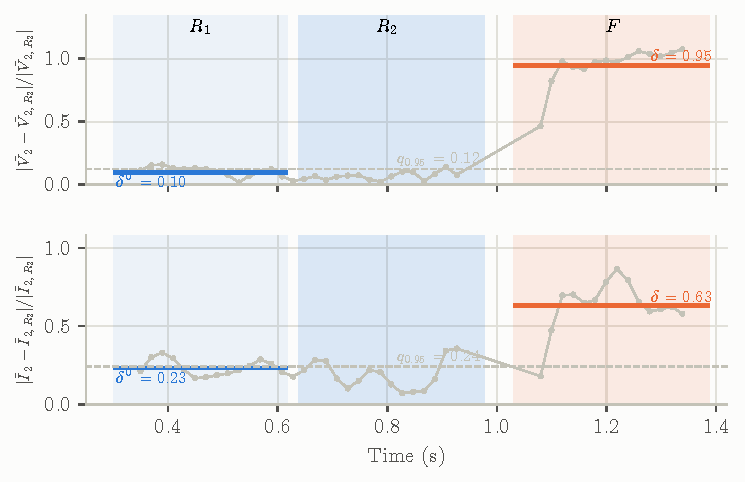
\includegraphics[width=\columnwidth]{G_sdr_illustration}
\caption{The SDR on one PMSG inter-turn trial (7.4\,\%, 1500\,rpm, 6.4\,N\,m): deviation of the voltage (top) and current (bottom) negative-sequence ratio from its $R_2$ mean; bars, $\delta^0$ and $\delta$; dashed, the machine's pooled $q_{0.95}$}\label{fig:sdrillu}
\end{figure}

The SDR is a mean-shift statistic with a known change time, standardised by an empirical quantile of its own drift null. For a scalar feature with a zero-mean Gaussian null, $q_{0.95}(|\delta^0|)=1.96\,\sigma_{\delta^0}$, and $\mathrm{SDR}\ge1$ would then be a two-sided 5\,\% test on the shift of interval means, the fixed-sample, known-onset case of the generalised likelihood ratio of \citet{Basseville1993}. For a phasor residual, the magnitude of a complex difference, the reference under a circular Gaussian null is a Rayleigh variable, whose 95\,\% point is 1.73 times the root-mean-square change. The empirical quantile lies within 3 to 11\,\% of these references for the fixed features of both machines (Section~\ref{sec:res-mde}), so the calibration is close to a parametric one. It is kept because it needs no shape choice per feature, and because the tails are heavier than the references, unevenly across speeds (Section~\ref{sec:res-mde}). The quantile is an estimate whose 95\,\% sampling interval spans a factor 1.3 to 1.5 here, and every interval reported resamples it with the numerator. Eq.~(\ref{eq:delta}) divides by the healthy level of the feature. A feature whose healthy level crosses zero has an unbounded null and is excluded by the screen below; the sequence residuals are normalised by the inherent asymmetry of the machine, which is bounded away from zero, and Section~\ref{sec:res-robust} reports the SDR in absolute units beside the relative form. With a known onset, a whole faulted interval averaged and a reference immediately before the fault, the SDR characterises the simplest detector on the feature: an abrupt-onset threshold at a stationary operating point against a null of sub-second variability. A detector that combines features or accumulates evidence can detect below $\mathrm{SDR}=1$, which is why the calibrated oracle and the transfer experiment are part of the method. Because a quieter null raises the SDR as much as a stronger signature does, numerator and denominator are reported separately when candidates are compared (Section~\ref{sec:res-where}).

\emph{Safeguards.} (i) On healthy trials the ``faulted'' interval contains only the switching operation, so a feature should exceed $\mathrm{SDR}=1$ there at the nominal rate $1-\alpha$. A feature whose false-alarm count in the $n_h$ healthy trials is incompatible with that rate (one-sided binomial test at the 5\,\% level; three or more of nine at $\alpha=0.95$), or whose null quantile exceeds one, is excluded for that candidate. With nine healthy trials the screen has little power (a true rate of 20\,\% passes with probability 0.74), so every false-alarm count is reported. (ii) A suite is evaluated by one \emph{fixed} feature, chosen once among its screened features by the smallest minimum detectable extent, then the detectable share, then the median SDR. The rule selects on the median-crossing extent, not on the power at a requirement, so a suite's adequacy below is adequacy under this prescribed univariate selection; Section~\ref{sec:res-suites} reports what a requirement-specific selection changes. The false-alarm count enters only through the screen, not as a tie-break, which is a choice: a design team may prefer the quieter of two features that tie on extent and share. It is also evaluated by the \emph{oracle} feature, the best feature of each trial, at a calibrated threshold: the $\alpha$-quantile of $\max_\varphi |\delta^0_\varphi|/q_\alpha(|\delta^0_\varphi|)$ over all records, because a maximum over $k$ features exceeds the single-feature threshold at a rate of up to $1-\alpha^k$. (iii) Every design quantity carries a bootstrap interval, over tap pairs for statements about a class and over the trials within an extent level for the limit-of-detection quantities, with the null quantile re-estimated in every resample.

\subsection{Derived quantities}\label{sec:derived}

For each candidate $a$, suite $s$ and class $f$, the \emph{diagnosability map} $D_a(s,f,e,o)$ is the SDR of the suite's fixed feature at extent $e$ and operating point $o$. Three limit-of-detection quantities are read from it on the tested extent levels, the physically distinct fault sizes of the test matrix (Section~\ref{sec:extent}). The \emph{minimum detectable extent} $\mathrm{MDE}_a(s,f)$ is the smallest tested level $e^\ast$ such that $\operatorname{median}_o D_a(s,f,e,o)\ge1$ for every tested $e\ge e^\ast$; it corresponds to a detection probability of about one half at $e^\ast$ and is reported as the bracket $(e^-, e^\ast]$ between the last undetected and the first detected level. The extent $e_{90}$ is the smallest tested level from which the \emph{detectable share} at the level itself, the fraction of its trials with $\mathrm{SDR}\ge1$, is at least 0.9 at that level and at every higher tested level; it is the $a_{90}$ of POD read on the tested grid, and the MDE and $e_{90}$ are reported as a pair because the gap between them reflects the slope of the POD curve (Section~\ref{sec:res-mde}). The \emph{bootstrap-supported} extent $e_{90}^{\mathrm{B}}$ is the smallest tested level from which that condition holds in at least 95\,\% of the resamples of Section~\ref{sec:procedure}. It is not the $a_{90/95}$ confidence bound of POD: the resampling fraction measures how stable the decision is under the procedure, with the feature re-selected and the null re-estimated, not the frequentist coverage of a detection probability, and with 36 trials at a level even 36 detections of 36 leave a one-sided 95\,\% binomial lower bound of 0.92 on the detection probability, with 18 of 18 one of 0.85. The share is assessed over the empirical mixture of operating points represented at each tested level, equal weights per trial, which is not a turbine duty cycle. The share may also be pooled over all tested levels at or above a requirement, $\mathrm{DS}_a(s,f\mid e\ge e_{\mathrm{req}})$; the pooled share depends on the composition of the matrix, so the share at the level is the operator-facing quantity and the pooled one is reported for comparison. The \emph{signature location} is the measurement group---stator currents, terminal voltages, controller internals, mechanical quantities, excitation---whose best screened feature attains the highest SDR in the largest share of trials. For a requirement $(f, e_{\mathrm{req}}, \alpha)$ the \emph{adequate} suites of a candidate are those that meet the joint condition of step~5 below at $e_{\mathrm{req}}$ itself, a local decision at the required extent; $e_{90}^{\mathrm{B}}$ summarises from which level that decision holds at every higher tested level too, so $e_{90}^{\mathrm{B}}\le e_{\mathrm{req}}$ implies adequacy but not conversely, and on these data the two coincide because no suite meets a level and fails a higher one (Section~\ref{sec:res-suites}); the signature location tells the designer \emph{why} a candidate behaves as it does. Table~\ref{tab:quantities} collects the quantities.

\begin{table*}[htbp]
\tabsize
\setlength{\tabcolsep}{4pt}
\centering
\caption{The quantities of the method: the statistic, the empirical performance read from it and the stability measures}\label{tab:quantities}
\begin{threeparttable}
\begin{tabular}{@{}L{2.9cm}L{1.5cm}L{2.2cm}L{6.2cm}@{}}
\toprule
Quantity & Symbol & Kind & Definition \\
\midrule
Signal-to-drift ratio & $\mathrm{SDR}$ & statistic, per trial & $|\delta|/q_\alpha(|\delta^0|)$, Eq.~(\ref{eq:sdr}); detection at $\mathrm{SDR}\ge1$ \\
Median SDR & -- & empirical performance & median over the trials of a level or a class; the numerator and denominator are reported separately when machines are compared \\
Minimum detectable extent & $\mathrm{MDE}$ & empirical performance & smallest tested level from which the median SDR is $\ge1$ at every level up; a bracket $(e^-, e^\ast]$ \\
Detectable share at a level & $\mathrm{DS}$ & empirical performance & fraction of the trials of a level with $\mathrm{SDR}\ge1$ (the POD estimate at that level) \\
Pooled share & $\mathrm{DS}(e\ge e_{\mathrm{req}})$ & empirical performance & the same over all tested levels at or above $e_{\mathrm{req}}$; depends on the test matrix \\
90\,\%-detection extent & $e_{90}$ & empirical performance & smallest tested level from which $\mathrm{DS}\ge0.9$ at every level up ($a_{90}$ on the tested grid) \\
Bootstrap-supported extent & $e_{90}^{\mathrm{B}}$ & stability & smallest level from which the $e_{90}$ condition holds in $\ge95\,\%$ of resamples; not a confidence bound \\
Bootstrap support & -- & stability & fraction of resamples in which a suite meets the requirement at $e_{\mathrm{req}}$ (step~5); meets $\ge0.95$, fails $\le0.05$ \\
Intervals & [lo, hi] & stability & percentile bootstrap over tap pairs (class statements) or over the trials of a level (limit-of-detection quantities), null re-estimated \\
Calibrated oracle & -- & empirical performance & best feature of each trial at the threshold calibrated for the maximum over the suite's features \\
\bottomrule
\end{tabular}
\end{threeparttable}
\end{table*}

\subsection{Procedure}\label{sec:procedure}

\begin{figure*}[htbp]
\centering
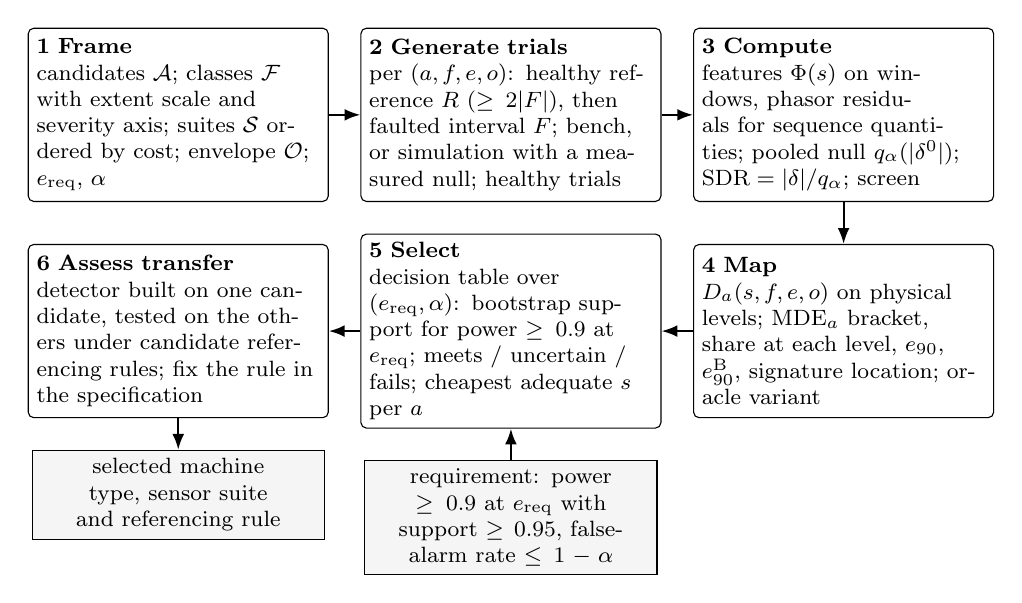
\begin{tikzpicture}[
  font=\footnotesize,
  box/.style={draw, rounded corners=2pt, align=left, inner sep=3pt, text width=3.6cm, minimum height=2.2cm},
  data/.style={draw, align=center, inner sep=3pt, text width=3.5cm, fill=black!4},
  arr/.style={-{Latex[length=2mm]}, thick},
  node distance=4mm and 4mm
]
\node[box] (s1) {\textbf{1 Frame}\\ candidates $\mathcal{A}$; classes $\mathcal{F}$ with extent scale and severity axis; suites $\mathcal{S}$ ordered by cost; envelope $\mathcal{O}$; $e_{\mathrm{req}}$, $\alpha$};
\node[box, right=of s1] (s2) {\textbf{2 Generate trials}\\ per $(a,f,e,o)$: healthy reference $R$ ($\ge 2|F|$), then faulted interval $F$; bench, or simulation with a measured null; healthy trials};
\node[box, right=of s2] (s3) {\textbf{3 Compute}\\ features $\Phi(s)$ on windows, phasor residuals for sequence quantities; pooled null $q_\alpha(|\delta^0|)$; $\mathrm{SDR}=|\delta|/q_\alpha$; screen};
\node[box, below=of s2] (s5) {\textbf{5 Select}\\ decision table over $(e_{\mathrm{req}},\alpha)$: bootstrap support for power $\ge0.9$ at $e_{\mathrm{req}}$; meets / uncertain / fails; cheapest adequate $s$ per $a$};
\node[box, right=of s5] (s4) {\textbf{4 Map}\\ $D_a(s,f,e,o)$ on physical levels; $\mathrm{MDE}_a$ bracket, share at each level, $e_{90}$, $e_{90}^{\mathrm{B}}$, signature location; oracle variant};
\node[box, left=of s5] (s6) {\textbf{6 Assess transfer}\\ detector built on one candidate, tested on the others under candidate referencing rules; fix the rule in the specification};
\draw[arr] (s1) -- (s2);
\draw[arr] (s2) -- (s3);
\draw[arr] (s3) -- (s4);
\draw[arr] (s4) -- (s5);
\draw[arr] (s5) -- (s6);
\node[data, below=4mm of s6] (out) {selected machine type, sensor suite and referencing rule};
\draw[arr] (s6) -- (out);
\node[data, below=4mm of s5] (req) {requirement: power $\ge0.9$ at $e_{\mathrm{req}}$ with support $\ge0.95$, false-alarm rate $\le 1-\alpha$};
\draw[arr] (req) -- (s5);
\end{tikzpicture}
\caption{The six-step procedure; steps 3--4 are fixed by Eqs.~(\ref{eq:delta})--(\ref{eq:sdr}), steps 1, 2, 5 and 6 follow the default rules of Section~\ref{sec:procedure}}\label{fig:method}
\end{figure*}

The procedure (Fig.~\ref{fig:method}) has six steps; steps 3--4 are fixed by Eqs.~(\ref{eq:delta})--(\ref{eq:sdr}), the others are design decisions with default rules.
\begin{enumerate}
  \item \textbf{Frame.} Enumerate $\mathcal{A}$, the classes $\mathcal{F}$ with an extent scale realisable in every candidate and a physical severity covariate, the suites $\mathcal{S}$ ordered by cost and the envelope $\mathcal{O}$. Set $e_{\mathrm{req}}$ as the smallest extent whose growth to an unacceptable consequence outpaces the inspection interval, $1-\alpha$ as the per-trial false-alarm rate tolerated, and the detection power. State whether the power is required on average over the envelope or at every operating point, the lowest monitored speed included. State whose cost ordering is used: controller access is cheap for the manufacturer of the converter and dear for a third-party retrofit.
  \item \textbf{Generate trials.} For each $(a,f,e,o)$ obtain trials with a healthy reference of at least twice the faulted duration immediately followed by the fault, covering at least the levels that bracket $e_{\mathrm{req}}$ and the corners of the envelope, plus healthy trials with the same timing for the screen.
  \item \textbf{Compute.} Extract $\Phi(s)$ on sliding windows within the intervals, form the pooled null per candidate and feature, compute the SDR per trial, apply the screen.
  \item \textbf{Map.} Build $D_a(s,f,e,o)$ and summarise it into $\mathrm{MDE}_a$, $e_{90}$, $e_{90}^{\mathrm{B}}$, $\mathrm{DS}_a$ and the signature location for the fixed and oracle variants, with bootstrap intervals.
  \item \textbf{Select.} Build the decision table. For each candidate, class, suite and $(e_{\mathrm{req}}, \alpha)$, count the resamples in which $\mathrm{MDE}\le e_{\mathrm{req}}$ and the share at the tested level that $e_{\mathrm{req}}$ maps to is at least the required power (0.9 here). Classify the suite as \emph{meets} when that fraction is at least 0.95, \emph{fails} when it is at most 0.05 and \emph{uncertain} otherwise. The fraction is resampling support, not a posterior probability and not a confidence level: a value of 1.00 means that no resample failed, and the table is an empirical assessment of how stable each decision is under the procedure. The decisions are conditional on the empirical pre-fault variability and on the available no-fault event screen; they do not independently verify a 5\,\% false-alarm rate under general operating disturbances. The fixed feature is re-selected and the null re-estimated in every resample; the trials of a level are resampled with its tap pairs treated as exchangeable, and the tap-pair unit is reported where the two differ. A suite's verdict is at least that of its subsets, and $e_{\mathrm{req}}$ takes the tested levels, because between levels the MDE is only a bracket. The adequate suite is the cheapest, under the stated cost ordering, that meets the requirement for every class.
  \item \textbf{Assess transfer.} If the detector must serve a family of candidates, test it across them under candidate feature-referencing rules; the rule that transfers enters the specification.
\end{enumerate}

\subsection{Scope, and the design-stage instantiation as outlook}\label{sec:design-stage}\label{sec:scope}

The method applies to classes that can be seeded at a known extent, at a stationary operating point, with a healthy interval immediately before the fault, in every candidate. That is a strong precondition, as it is for POD, and it is the price of needing no model. The method evaluates a threshold on interval means, not the time to detection. The level $1-\alpha$ is a per-decision rate: at one decision per interval (0.36\,s here) $\alpha=0.95$ is a false alarm every 7\,s, so the MDEs reported are bench limits of detection, not field thresholds, and a field monitor needs an accumulation rule over many decisions (Section~\ref{sec:implications}). As an outlook, not tested here, the two ingredients of the SDR could be supplied separately before hardware exists: the numerator by a finite-element or circuit model of each candidate with the fault injected \citep{Vaseghi2009}, validated on a few physical trials, and the denominator from measured healthy records of hardware of the same class. That rests on the assumption that the healthy variability depends on the sensing and control chain more than on the machine, which Section~\ref{sec:res-where} tests on two machines of one bench.
%% ----------------------------------------------------------------------
%% demo
%% ----------------------------------------------------------------------

\section{Demonstration on three wind-turbine generator--drive systems}\label{sec:demo}

\subsection{Machines and data}\label{sec:data}

The three candidates are laboratory-scale generators on instrumented test benches at the University of S\~ao Paulo, published as open benchmark datasets (Table~\ref{tab:alternatives}, Fig.~\ref{fig:alternatives}). The PMSG \citep{Tominaga2025pmsg} and the SCIG \citep{Tominaga2025scig} are four-pole, 230\,V, double-star machines rated 2.5\,kVA and 2.5\,kW, on the \emph{same} bench. They share the prime mover, the converter, the control platform and the field-oriented control (FOC; rotor angle from an encoder for the PMSG, from a flux observer for the SCIG), the sensors, the acquisition (20\,kHz, 3\,s records), the fault-insertion hardware and the test script. Everything but the machine and the control structure it requires is therefore held fixed. The variable-speed WFSG \citep{Tominaga2024gen} is a 2\,kVA four-salient-pole machine on an earlier bench of the same group \citep{Rocha2023}, with a three-level converter, FOC with encoder angle, 4\,kHz acquisition and 1.3\,s records. It carries the same tapped short-circuits on a different bench, whose fault resistances, fault durations, converter, sampling rate and voltage sensing all differ, and its variable-speed dataset holds no healthy records, so the screen and the nuisance-transient negatives are unavailable for it. The PMSG--SCIG pair is therefore the controlled comparison of this paper; the WFSG is an extension with a different evidential status, marked as such in every table. The data papers state neither the loop gains nor the switching frequencies, observer structure or transducer bandwidths.

\begin{table*}[htbp]
\tabsize
\setlength{\tabcolsep}{4pt}
\centering
\caption{The three candidate systems; the PMSG and SCIG share one bench and one protocol, the WFSG bench differs where indicated}\label{tab:alternatives}
\begin{threeparttable}
\begin{tabular}{@{}L{2.4cm}L{2.8cm}L{3.3cm}L{3.4cm}@{}}
\toprule
 & PMSG & SCIG & WFSG (variable speed) \\
\midrule
Rating, poles & 2.5\,kVA, 4 & 2.5\,kW, 4 & 2\,kVA, 4 salient \\
Rated current & 6.3\,A & 7.7\,A & not stated \\
Excitation & permanent magnets & induction (magnetising current) & wound field, static exciter \\
Converter and control & 2L, FOC with encoder & 2L, FOC with flux observer & 3L-NPC, FOC with encoder \\
Acquisition & 20\,kHz, 3\,s & 20\,kHz, 3\,s & 4\,kHz, 1.3\,s \\
Reference / faulted interval & 0.68\,s / 0.36\,s & 0.68\,s / 0.36\,s & 0.49\,s / 0.06--0.28\,s \\
Fault resistance & 2.6\,$\Omega$ & 2.6\,$\Omega$ & 1, 2.83, 5.66, 11.32\,$\Omega$ \\
Operating points & 3 speeds $\times$ 3 torques & same & 716--1910\,rpm, 4 torque levels (sparse) \\
Healthy trials & 9 & 9 & none \\
Fault trials & 216 & 216 & 438 (198 at 2.83\,$\Omega$) \\
\bottomrule
\end{tabular}
\begin{tablenotes}[flushleft]
\item Ratings as given by the manufacturer (kVA for the synchronous machines, kW for the induction machine). 2L: two-level converter; 3L-NPC: three-level neutral-point-clamped converter; FOC: field-oriented control. Current-loop gains and bandwidths, switching frequencies and the flux-observer structure are not given in the data papers.
\end{tablenotes}
\end{threeparttable}
\end{table*}

\begin{figure*}[htbp]
\centering
\definecolor{pmsgc}{HTML}{2A78D6}
\definecolor{scigc}{HTML}{EB6834}
\definecolor{wfsgc}{HTML}{1BAF7A}
\begin{tikzpicture}[
  font=\small, x=1cm, y=1cm, line cap=round, line join=round,
  frame/.style={draw=black!70, line width=0.8pt},
  hd/.style={anchor=south, inner sep=1pt},
  sub/.style={anchor=north, inner sep=1pt, text width=12.6cm, align=center}
]
%% One row per alternative: turbine rotor, shaft, generator (stator ring with the rotor symbol),
%% three-phase stator connection, back-to-back converter (ac/dc, dc link, dc/ac) and grid.
\newcommand{\chain}[1]{%
  \foreach \ang in {90,210,330} {
    \begin{scope}[shift={(1.1,#1)}, rotate=\ang-90]
      \path[frame, fill=black!15] (0.07,0) .. controls (0.18,0.22) and (0.13,0.52) .. (0,0.7)
                                   .. controls (-0.13,0.52) and (-0.18,0.22) .. (-0.07,0) -- cycle;
    \end{scope}
  }
  \fill[black!70] (1.1,#1) circle (0.09);
  \draw[black!55, line width=2.2pt] (1.25,#1) -- (3.7,#1);
  \filldraw[frame, fill=black!8] (4.3,#1) circle (0.62);
  \filldraw[frame, fill=white] (4.3,#1) circle (0.5);
  \draw[frame] (4.92,#1) -- (7.2,#1);
  \foreach \s in {-0.09,0,0.09} { \draw[frame] (6.0+\s,#1-0.12) -- (6.14+\s,#1+0.12); }
  \filldraw[frame, fill=black!5] (7.2,#1-0.4) rectangle (8.0,#1+0.4);
  \draw[frame] (7.2,#1-0.4) -- (8.0,#1+0.4);
  \node[inner sep=0] at (7.41,#1+0.2) {$\sim$};
  \node[inner sep=0] at (7.79,#1-0.2) {$=$};
  \draw[frame] (8.0,#1+0.1) -- (8.3,#1+0.1);
  \draw[frame] (8.0,#1-0.1) -- (8.3,#1-0.1);
  \filldraw[frame, fill=black!5] (8.3,#1-0.4) rectangle (9.1,#1+0.4);
  \draw[frame] (8.3,#1-0.4) -- (9.1,#1+0.4);
  \node[inner sep=0] at (8.51,#1+0.2) {$=$};
  \node[inner sep=0] at (8.89,#1-0.2) {$\sim$};
  \draw[frame] (9.1,#1) -- (11.3,#1);
  \draw[black!70, line width=2.4pt] (11.3,#1-0.5) -- (11.3,#1+0.5);
}
%% column headers
\node[hd] at (1.1,0.85) {turbine rotor};
\node[hd] at (4.3,0.85) {generator};
\node[hd] at (8.15,0.85) {converter};
\node[hd] at (11.3,0.85) {grid};
%% (a) PMSG: permanent magnets on the rotor surface
\chain{0}
\draw[black!50, line width=0.6pt] (4.3,0) circle (0.31);
\foreach \a in {0,120,240} { \draw[pmsgc, line width=2.8pt] (4.3,0) ++(\a+7:0.4) arc[start angle=\a+7, end angle=\a+53, radius=0.4]; }
\foreach \a in {60,180,300} { \draw[black!40, line width=2.8pt] (4.3,0) ++(\a+7:0.4) arc[start angle=\a+7, end angle=\a+53, radius=0.4]; }
\node[sub] at (6.2,-0.8) {(a) PMSG};
%% (b) SCIG: squirrel cage
\chain{-2.1}
\draw[scigc, line width=1.1pt] (4.3,-2.1) circle (0.42);
\draw[scigc, line width=1.1pt] (4.3,-2.1) circle (0.26);
\foreach \a in {0,30,...,330} { \draw[scigc, line width=1.1pt] (4.3,-2.1) ++(\a:0.26) -- ++(\a:0.16); }
\node[sub] at (6.2,-2.9) {(b) SCIG};
%% (c) WFSG: field winding on the rotor
\chain{-4.2}
\draw[black!50, line width=0.6pt] (4.3,-4.2) circle (0.42);
\draw[wfsgc, line width=1.1pt, decorate, decoration={coil, aspect=0.6, segment length=1.9mm, amplitude=1.9mm}] (3.9,-4.2) -- (4.7,-4.2);
\node[sub] at (6.2,-5.0) {(c) WFSG};
\end{tikzpicture}
\caption{The three candidates as generator systems: turbine rotor, generator with its rotor excitation (cage, field winding or magnets), converter and grid}\label{fig:alternatives}
\end{figure*}

\subsection{Failure-mode class and extent scale}\label{sec:extent}

All three machines have 24 tapped derivation points at the same relative positions of their stator windings. Two classes are used (Fig.~\ref{fig:faults}): inter-turn short-circuits (both taps on one branch) and inter-winding short-circuits (taps on the two parallel branches of a phase). The extent $e$ is the fraction of a branch between the taps, 2.7--12.1\,\% for the twelve inter-turn and 2.3--40.2\,\% for the twelve inter-winding cases. The nominal extents overstate the resolution of the matrix. The fault current of a resistor-limited short-circuit is set by the voltage induced in the shorted turns, so tap pairs with equal fault currents short the same number of turns and are the same physical fault: on the PMSG the four pairs of each inter-turn level carry fault currents within 3\,\% of each other (1.4, 3.8 and 6.0\,A), and the SCIG currents cluster within 8\,\%. In per unit of the nameplate current (6.3\,A for the PMSG, 7.7\,A for the SCIG) the three inter-turn levels carry 0.23, 0.60 and 0.96 (PMSG) and 0.15, 0.44 and 0.73 (SCIG), and the inter-winding levels 0.33 to 2.8 and 0.25 to 2.0; that scale compares the machines but not the fault physics, which the fault-to-stator ratio of Section~\ref{sec:res-where} carries. The limit-of-detection quantities are therefore evaluated on \emph{physical extent levels}, tap pairs of one class whose median fault currents, normalised per machine and averaged over the two machines, lie within 7\,\% of the first pair of the level. There are three inter-turn levels (2.7--3.8, 7.4--7.7 and 11.6--12.1\,\% of a branch) and six inter-winding levels (2.3--3.2, 9.7--10.6, 14.3--14.8, 21.7--22.2, 33.7--37.5 and 40.2\,\%). The tap layout has a second property that matters for sequence features. The four smallest inter-turn pairs lie in phase A, the 7.4--7.7\,\% pairs in phases A and B and the largest in phases A and C, so on the nominal extent axis the faulted phase is confounded with the extent (Section~\ref{sec:res-phase}). Faults were closed through a contactor and a series resistance at steady state: 2.6\,$\Omega$ for 0.4\,s on the PMSG and SCIG, and 1 to 11.32\,$\Omega$ on the WFSG, where the resistance was raised with extent, so that extent and impedance are confounded on that bench. The severity is \emph{resistor-limited}, unlike a bolted fault, which the leakage reactance of the shorted turns limits.

\begin{figure*}[htbp]
\centering
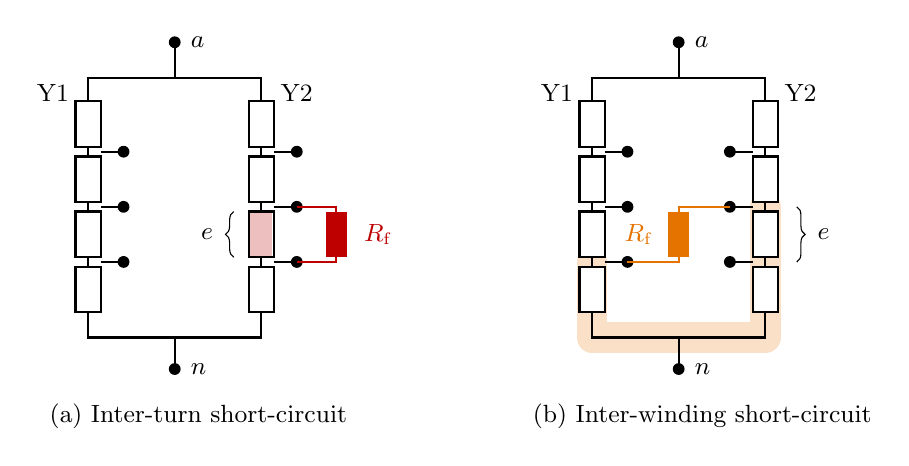
\begin{tikzpicture}[
  font=\small, x=1cm, y=1cm,
  wire/.style={thick},
  coil/.style={draw, thick, fill=white, minimum width=3.2mm, minimum height=5.8mm, inner sep=0},
  tap/.style={circle, fill=black, inner sep=0, minimum size=1.5mm},
  rf/.style={draw, thick, fill=white, minimum width=2.4mm, minimum height=5.5mm, inner sep=0},
  it/.style={red!75!black},
  iw/.style={orange!90!black}
]
%% One phase (a--n) of the double-star stator: two parallel branches Y1 and Y2 of four coil groups with
%% tapped derivation points. Panel (a) inter-turn fault, panel (b) inter-winding fault.
\foreach \dx in {0, 6.4} {
  % circulating path of the inter-winding fault (panel b only), drawn first so that it lies behind
  \ifdim \dx pt > 1pt
    \draw[iw, line width=11pt, line cap=round, line join=round, opacity=0.22]
      (\dx+0.9,1.71) -- (\dx+0.9,0.75) -- (\dx+3.1,0.75) -- (\dx+3.1,2.41);
  \fi
  % terminal, junctions, branches, neutral
  \node[tap, label={right:$a$}] at (\dx+2.0,4.5) {};
  \draw[wire] (\dx+2.0,4.5) -- (\dx+2.0,4.05) -- (\dx+0.9,4.05) -- (\dx+0.9,0.75) -- (\dx+2.0,0.75) -- (\dx+2.0,0.35);
  \draw[wire] (\dx+2.0,4.05) -- (\dx+3.1,4.05) -- (\dx+3.1,0.75) -- (\dx+2.0,0.75);
  \node[tap, label={right:$n$}] at (\dx+2.0,0.35) {};
  \node[anchor=east] at (\dx+0.78,3.85) {Y1};
  \node[anchor=west] at (\dx+3.22,3.85) {Y2};
  \foreach \bx in {0.9, 3.1} {
    \foreach \cy in {3.46, 2.76, 2.06, 1.36} { \node[coil] at (\dx+\bx,\cy) {}; }
  }
  % taps of Y1 point into the gap between the branches
  \foreach \ty in {3.11, 2.41, 1.71} {
    \draw[wire] (\dx+1.06,\ty) -- (\dx+1.35,\ty); \node[tap] at (\dx+1.35,\ty) {};
  }
}
%% (a) inter-turn: two taps of one branch (Y2) shorted through R_f; the shorted coil group is shaded
\begin{scope}
  \foreach \ty in {3.11, 2.41, 1.71} {
    \draw[wire] (3.26,\ty) -- (3.55,\ty); \node[tap] at (3.55,\ty) {};
  }
  \fill[it, opacity=0.25] (2.96,2.33) rectangle (3.24,1.79);
  \draw[it, thick] (3.55,2.41) -- (4.05,2.41) -- (4.05,1.71) -- (3.55,1.71);
  \node[rf, it] at (4.05,2.06) {};
  \node[it, anchor=west] at (4.28,2.06) {$R_{\mathrm{f}}$};
  \draw[decorate, decoration={brace, amplitude=3pt}] (2.75,1.77) -- (2.75,2.35) node[midway, left=4pt] {$e$};
  \node at (2.3,-0.25) {(a) Inter-turn short-circuit};
\end{scope}
%% (b) inter-winding: a tap of Y1 and a tap of Y2 at different positions shorted through R_f;
%% the fault current circulates through the lower parts of both branches and the neutral link
\begin{scope}[shift={(6.4,0)}]
  \foreach \ty in {3.11, 2.41, 1.71} {
    \draw[wire] (2.94,\ty) -- (2.65,\ty); \node[tap] at (2.65,\ty) {};
  }
  \draw[iw, thick] (1.35,1.71) -- (2.0,1.71) -- (2.0,2.41) -- (2.65,2.41);
  \node[rf, iw] at (2.0,2.06) {};
  \node[iw, anchor=east] at (1.8,2.06) {$R_{\mathrm{f}}$};
  \draw[decorate, decoration={brace, mirror, amplitude=3pt}] (3.5,1.71) -- (3.5,2.41) node[midway, right=4pt] {$e$};
  \node at (2.3,-0.25) {(b) Inter-winding short-circuit};
\end{scope}
\end{tikzpicture}
\caption{Inter-turn (\textbf{a}) and inter-winding (\textbf{b}) short-circuits through $R_{\mathrm{f}}$ between taps of one phase of the double-star stator; $e$ is the fraction of a branch between the taps}\label{fig:faults}
\end{figure*}

The PMSG and SCIG matrix is complete: 24 fault cases $\times$ 3 speeds (1200, 1500, 1800\,rpm) $\times$ 3 torques (5.2, 6.4, 8.0\,N\,m, 39--60\,\% of rated torque), scaled from the operating region of the International Energy Agency 15\,MW reference turbine \citep{Gaertner2020} by the speed ratio, plus the healthy condition at each operating point; the SCIG generates with slip, at 59.6\,Hz at 1800\,rpm. The WFSG matrix covers the same 24 tap pairs at six speeds (716--1910\,rpm) and four torque levels, sparsely. The analyses use the WFSG's 438 inter-turn and inter-winding trials at all impedances for the null and the feature ranking, with the impedance as a covariate, and the 198 trials at 2.83\,$\Omega$, the impedance closest to the PMSG/SCIG value, covering four inter-turn pairs of 11.6--12.1\,\% and four inter-winding pairs of 2.3--10.6\,\%, for the MDE and the decision table.

\subsection{Sensor suites and features}\label{sec:suites}

Five sensor suites are considered, ordered by the data access, hardware and integration they add to a bare generator--converter set (Table~\ref{tab:suitedef}). \emph{Drive-internal} uses only quantities the converter controller already has. \emph{3\,CT} uses the three phase currents with angle-free features, so that its cost is data access rather than hardware. \emph{3\,CT + 3\,VT} adds three terminal voltage transducers (VT), \emph{3\,CT + 3\,VT + drive} adds controller access, and \emph{+ torque transducer} adds a shaft torque sensor. For the WFSG the field current is an additional drive-internal observable (the \emph{excitation} suite), available because its exciter is static \citep{Neti2009}. The ordering is the one of a converter manufacturer; a third-party retrofit reads it from 3\,CT upward (Section~\ref{sec:implications}). Sequence quantities enter in two forms. The magnitude ratios $I_2/I_1$, $V_2/V_1$ and $D_2/D_1$ of currents, terminal voltages and duty cycles are the established indicators \citep{Kliman1996, Lee2003, Cruz2001}. The phasor residuals $|\Delta\bar I_2|/I_1$, $|\Delta\bar V_2|/V_1$ and $|\Delta\bar D_2|/D_1$ are the magnitude of the change of the complex negative-sequence component referenced to the positive-sequence angle, which isolates the fault-induced part whatever the faulted phase \citep{Kliman1996, Arkan2001}. With $X_+$ and $X_-$ the symmetrical components of the Hann-windowed complex amplitudes of the three phase signals at $f_e$, the phase-referenced ratio of a window is $\bar X_2 = X_-\overline{X_+}/|X_+|^2$, whose angle does not rotate with the window start. The feature label $|\Delta\bar X_2|/X_1$ names this ratio to the positive sequence; its relative changes in Eq.~(\ref{eq:delta}) are then $|\bar X_{2,F}-\bar X_{2,R_2}|/|\bar X_{2,R_2}|$ under fault and $|\bar X_{2,R_2}-\bar X_{2,R_1}|/|\bar X_{2,R_1}|$ in the null, so the SDR of a residual feature divides a change of the negative sequence by a quantile of its healthy changes, both relative to the machine's inherent asymmetry. Features are computed on sliding windows of $n_c$ electrical cycles with a hop of one cycle. The electrical frequency and the phase rotation are estimated per window from the slope of the unwrapped phase of the current space vector, so that the external suites need no angle sensor. The other features are the standard deviation of the mean-removed signal and its amplitudes at $f_e$ and $2f_e$ as listed in Table~\ref{tab:suitedef}. On the WFSG bench the converter-side phase voltages serve as terminal voltages and the electrical torque is computed from power and speed.

\begin{table*}[htbp]
\tabsize
\setlength{\tabcolsep}{4pt}
\centering
\caption{Sensor suites and the features they can compute}\label{tab:suitedef}
\begin{threeparttable}
\begin{tabular}{@{}L{2.3cm}L{3.0cm}L{7.0cm}@{}}
\toprule
Suite & Added access / hardware & Features \\
\midrule
Drive-internal & controller data & $I_d, I_q$: std, 1$f_e$, 2$f_e$; $V_d^{\mathrm{cmd}}, V_q^{\mathrm{cmd}}$: 2$f_e$; PI outputs $d,q$: std, 2$f_e$; duty-cycle negative sequence $D_2/D_1$; $T_e$: std, 1$f_e$, 2$f_e$; DC-link std; speed std \\
3\,CT & three phase currents, no angle & $I_2/I_1$, RMS unbalance, harmonics 3, 5, 7 of $I_a$ relative to the fundamental, THD \\
3\,CT + 3\,VT & + 3 voltage transducers & 3\,CT features + $V_2/V_1$ \\
3\,CT + 3\,VT + drive & + controller data & all of the above + measured $V_d, V_q$: 2$f_e$ \\
+ torque transducer & + shaft torque sensor & + $T_m$: std, 1$f_e$, 2$f_e$ \\
Excitation (WFSG) & field-current measurement & $I_f$: std, 2$f_e$ \\
\bottomrule
\end{tabular}
\begin{tablenotes}[flushleft]
\item $f_e$: electrical frequency; 1$f_e$, 2$f_e$: amplitude of the component at once and twice the electrical frequency; $I_1, I_2$ ($V_1, V_2$): positive- and negative-sequence magnitudes at $f_e$; std: standard deviation; THD: total harmonic distortion; PI: proportional--integral.
\end{tablenotes}
\end{threeparttable}
\end{table*}

\subsection{Computation}\label{sec:computation}

For the PMSG and SCIG the reference interval is the 0.68\,s before the contactor command, split into $R_1$ (0.32\,s) and $R_2$ (0.36\,s). The faulted interval runs from 30\,ms after the command to 10\,ms before its release; the relay picks up 85--90\,ms after the command, so the interval holds about 55\,ms of healthy time, and Section~\ref{sec:res-robust} quantifies the effect. For the WFSG the fault interval starts where the 10\,ms RMS of the measured fault current first exceeds $\max(0.3\,\mathrm{A}, 6\sigma)$ and the reference interval (0.49\,s) is split at 0.30\,s; four trials with no complete fault window are dropped. A window belongs to $R_1$ when it ends before the split time and to $R_2$ when it starts after it. The reference intervals fall 6\,\% (common bench) and up to 13\,\% (longest WFSG faults) short of the twice-the-fault-duration rule of step~2. The main PMSG--SCIG comparison uses $n_c=5$; the three-machine comparison uses $n_c=3$ because the WFSG fault intervals are short; the sensitivity of every conclusion to $n_c\in\{3,5,8\}$ and $\alpha\in\{0.90,0.95,0.99\}$ is reported. The null is pooled over all 225 records of each of the PMSG and SCIG and over the 438 WFSG records. Bootstrap intervals use 2000 resamples: the median SDR and the pooled share of a class are resampled over the twelve tap pairs, the same pairs for both machines so that the SCIG/PMSG ratio is matched; the MDE and the share at a level over the trials within the level; and in every resample the null quantile is re-estimated from a cluster resample of the machine's 25 clusters. The decision table uses 10\,000 resamples per suite, candidate and class at $\alpha=0.95$ on the common bench and 1000 otherwise, with $e_{\mathrm{req}}$ at the tested levels and a required power of 0.9.

Step~6 is instantiated as a window-level change detector on all features of Table~\ref{tab:suitedef} that a machine provides. A gradient-boosted decision-tree (GBDT) classifier \citep{Friedman2001} is used because it handles features of different scales and shapes without tuning and makes no linearity assumption; a logistic regression is run beside it for the PMSG--SCIG pair as the linear comparator. Both are trained to separate faulted windows from healthy ones, within a machine by five-fold cross-validation grouped by tap pair and across machines by training on all trials of one machine and testing on all trials of another. Four feature-referencing rules are compared, and they correspond to three deployment scenarios. Physical units need no target data. Features $z$-scored on all healthy trials of the target machine, or on the healthy trial at the same operating point, need a commissioning record of the target. The absolute $z$-score of each window against the \emph{first half} of its own trial's reference interval needs only the immediately preceding healthy interval, which is the SDR's referencing assumption. Negatives are the reference and recovery windows of all trials plus the fault-interval windows of the healthy trials (141 and 140 of about 21\,000 out-of-reference windows on the PMSG and SCIG), the only negatives that contain the contactor operation without a fault; the recovery windows carry the release transient and are kept as negatives for that reason. Because the normalising windows are trivially separable under the fourth rule, every metric is reported on the out-of-reference windows, with 95\,\% intervals from 500 cluster resamples of the tested machine's trials. The GBDT is a histogram gradient boosting of depth 3 with 200 iterations at a learning rate of 0.08, the logistic regression is standardised with $C=1$, the within-machine folds are grouped by tap pair (healthy trials by speed), and the normalising set of the self-referenced rule is the windows ending before 0.62\,s (PMSG/SCIG) or 0.30\,s (WFSG).
%% ----------------------------------------------------------------------
%% results
%% ----------------------------------------------------------------------

\section{Results}\label{sec:results}

\subsection{The same design-level fault is not the same physical fault}\label{sec:res-severity}

For the same tap pair the SCIG's fault current is about 10\,\% lower than the PMSG's (medians 3.3 against 3.7\,A for inter-turn and 7.7 against 8.5\,A for inter-winding pairs). Relative to what the stator sensors see the difference is larger. The fault current is 1.45 times the pre-fault stator current (RMS, median over pairs) in the PMSG and 0.63 times in the SCIG for inter-turn faults, and 3.3 against 1.5 times for inter-winding faults, because the SCIG's stator current carries the magnetising component (5.3 against 2.6\,A RMS before the fault). The WFSG pairs at the matching impedance give 4.7 and 3.1, that bench running at a stator current of 1.1\,A. A fault specified as ``$e$\,\% of a winding'' therefore arrives at the sensors of the three machines as three different physical events. The ratio of fault current to stator current orders faults of equal turns correctly within a machine, because the magnetomotive force (MMF) asymmetry of a turn fault scales with the fault current times the shorted fraction, but it is confounded by the magnetising component across machines; it is kept as a covariate that exposes the distinction between design-level extent and physical severity, not as a scale that compares the machines (Section~\ref{sec:res-mde}).

\subsection{Where the signature appears, and why the SDR differs}\label{sec:res-where}

The null of the SDR differs between the PMSG and the SCIG on every feature, and by how much depends on the form in which the feature is written. In the relative form of Eq.~(\ref{eq:delta}) the SCIG's null is 2.4 times quieter than the PMSG's for the voltage residual, 5.2 times for the current residual and 45 times for the $d$-axis current ripple. In the units of the features themselves the factors are 1.1, 6.0 and 7.0, because the SCIG's healthy $d$-axis ripple is five times the PMSG's: its inherent negative-sequence current is 2.9 times the PMSG's in amperes (0.043 against 0.015\,A), and the flux-observer angle, modulated at 2$f_e$, is the plausible remainder. The decomposition of the SCIG/PMSG ratio of median SDR therefore reads differently for the three measurement groups. Through the terminal-voltage residual the machines are equivalent, numerator and null agreeing in volts to within 20\,\%. Through the stator-current residual the SCIG's SDR is 3.7 and 3.3 times the PMSG's while the PMSG's current change is the larger in both forms, so there the SCIG wins entirely by a quieter null. Through the $d$-axis features the SCIG's SDR is 16 and 23 times the PMSG's, and in absolute units the SCIG has both the larger signature and the quieter null. The reading that the SCIG wins only by silence thus holds for the stator current and is, for the controller quantities, an artefact of the relative normalisation. Nor is the null a property of the transducers alone, since the duty-cycle residual, a controller output, has a null 8.5 (relative) and 3.1 (absolute) times larger on the PMSG.

Fig.~\ref{fig:features} shows the median SDR of every feature for the three machines on three-cycle windows. In the PMSG the terminal-voltage group carries the strongest signature in 94\,\% of inter-turn and 97\,\% of inter-winding trials, through the voltage residual (median SDR 6.8 and 53 at five-cycle windows; 88 and 100\,\% of trials detectable), and the stator-current residual is weak for inter-turn faults (1.7; 70\,\%). In the SCIG the controller group is strongest in 63 and 67\,\% of trials, through the duty-cycle residual for inter-turn faults (11.2; 93\,\%) and the $d$-axis ripple and its PI output for inter-winding faults (68; 100\,\%), the stator-current group in 34 and 33\,\%. In the WFSG the terminal-voltage and current residuals, the commanded $q$-axis voltage and the field-current 2$f_e$ ripple, an observable the other two lack, are strongest. The physical quantity behind the relocation is the incremental negative-sequence impedance at the terminals, $\Delta\bar V_2/\Delta\bar I_2$ per trial: 12.7 [11.1, 14.1]\,$\Omega$ (inter-turn) and 12.2 [10.2, 13.2]\,$\Omega$ (inter-winding) in the PMSG against 7.3 [6.9, 7.7] and 7.4 [7.2, 7.6]\,$\Omega$ in the SCIG (medians and interquartile ranges), 0.60 and 0.35 per unit on the 2.5\,kVA, 230\,V base. The PMSG drive thus converts a negative-sequence current disturbance into 1.7 times the terminal voltage that the SCIG drive does. With the converter connected directly to the stator, this ratio is the closed-loop output impedance of the current regulator at the negative-sequence frequency \citep{Tallam2003, Cheng2011}. It is flat over the tested frequencies (Section~\ref{sec:res-robust}), as expected when the proportional gain dominates at $2f_e$; under the usual tuning $K_p\approx L\,\omega_{\mathrm{bw}}$ the ratio 1.7 would then be the ratio of the inductances the two regulators were tuned to for a common bandwidth, a hypothesis that the undocumented gains and inductances of the benches leave untested. The 2$f_e$ ripple of the synchronous-frame currents is the same negative-sequence current seen in the rotating frame, so the current and controller groups differ by normalisation and angle source rather than by physics. Both machines run the same field-oriented controller but differ in angle source, output impedance and healthy baselines, so the relocation belongs to the machine--drive combination, not to the control structure alone.

\begin{figure*}[htbp]
\centering
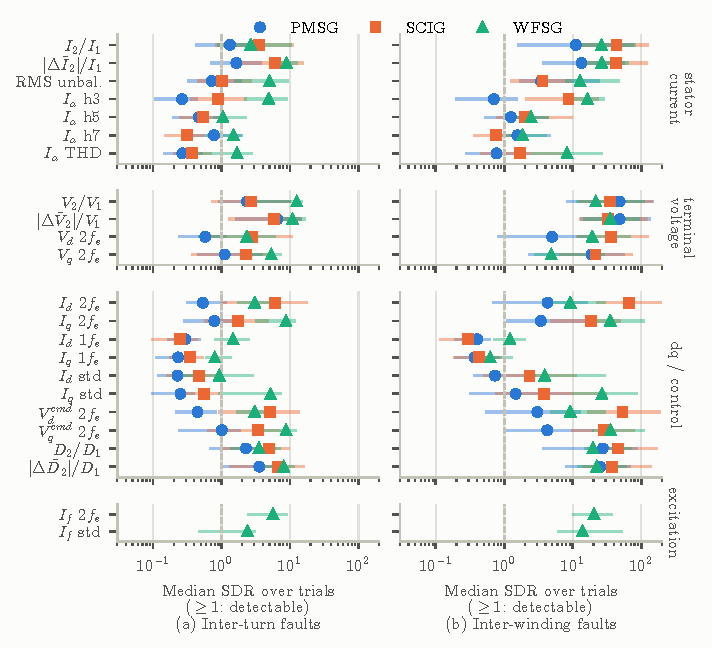
\includegraphics[width=\textwidth]{G_sdr_by_feature_3alt_compact}
\caption{Median SDR (dot) and interquartile range (bar) of every feature, three machines, three-cycle windows; the WFSG is unscreened and pooled over its fault impedances}\label{fig:features}
\end{figure*}

\subsection{The faulted phase and the extent axis}\label{sec:res-phase}

The inter-turn test matrix carries a second variable on its nominal extent axis: the four pairs of the smallest level lie in phase A, those of the middle level in phases A and B, those of the largest in phases A and C. Fig.~\ref{fig:pairs} shows why this matters. The magnitude ratios $V_2/V_1$ and $I_2/I_1$ depend on the faulted phase far beyond what the extents explain; the spread between the pairs of one level is a factor 3.8 to 14 for $V_2/V_1$ and 1.3 to 7 for $I_2/I_1$. The phasor residuals remove this almost entirely, the pairs of every level agreeing to within a factor 1.1 to 1.8 on both machines. The mechanism is the one of Section~\ref{sec:suites}. The inherent negative-sequence component of each machine is of the same order as the fault-induced one for a small inter-turn fault, so the magnitude of their sum rises or falls with the angle between them, which rotates by $\pm120^\circ$ with the faulted phase; the complex change does not. Hence the residual features represent the suites wherever a sequence quantity is used (Tables~\ref{tab:mde}--\ref{tab:decision}), the magnitude ratios remaining in Fig.~\ref{fig:features} as the established indicators. On the residual features the two machines on the common bench are nearly indistinguishable through the terminal voltage, with per-level medians of $|\Delta\bar V_2|/V_1$ of 1.1, 6.8 and 19.5 (PMSG) against 0.9, 6.9 and 19.5 (SCIG) at the three inter-turn levels, and they differ through the stator current, where the SCIG's residual is 2 to 4 times the PMSG's. The relocation of the signature survives the change of feature; the earlier reading that the PMSG's voltage signature is stronger than the SCIG's does not.

\begin{figure*}[htbp]
\centering
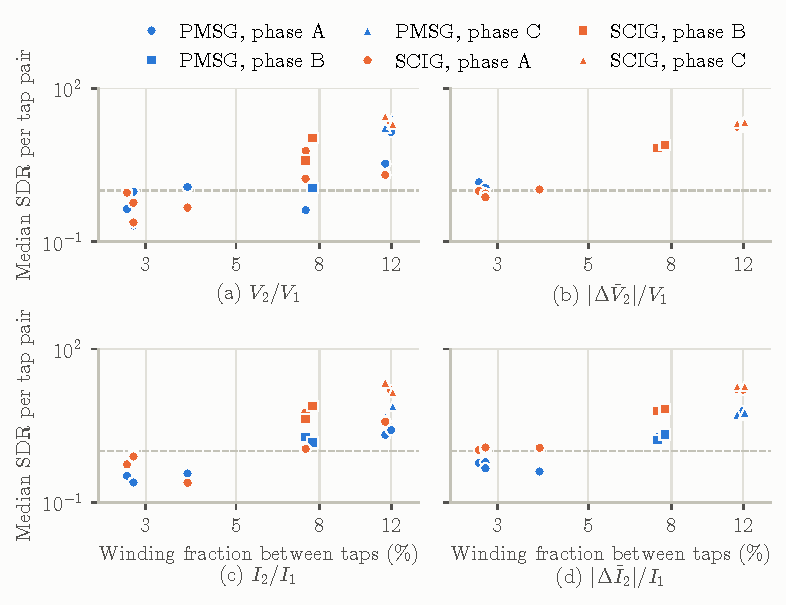
\includegraphics[width=\textwidth]{G_pairs_by_phase}
\caption{Inter-turn median SDR per tap pair against the nominal extent, five-cycle windows: magnitude ratios (\textbf{a}, \textbf{c}), phasor residuals (\textbf{b}, \textbf{d}); marker, phase; colour, machine}\label{fig:pairs}
\end{figure*}

\subsection{Minimum detectable extent and detection probability}\label{sec:res-mde}

Table~\ref{tab:mde} gives, for the two residual features, the $d$-axis PI ripple and the $q$-axis voltage ripple, the MDE as a bracket on the physical levels with its interval, the pooled detectable share and the median SDR with intervals from the tap-pair bootstrap, and the SCIG/PMSG ratio of medians. Fig.~\ref{fig:pod} gives the detection probability on the tested grid: the share at each level with its interval for the fixed features of the two machines. Through the terminal-voltage residual the PMSG detects every inter-turn level including the smallest by the median criterion (per-level median SDR 1.1; share 64\,\% at that level, 88\,\% [74, 98] pooled) and the SCIG every level from the middle one (its smallest level sits at a median of 0.9). Through the stator-current residual the point estimates reverse, while the intervals of both MDEs span the two smallest levels. The $d$-axis ripple detects from the middle level on the SCIG and only the largest on the PMSG. With power 0.9 the picture is simpler: no feature of either machine reaches $e_{90}$ at the smallest inter-turn level (shares at the level 11 to 78\,\%), and every fixed feature reaches it at the middle level, where every trial is detected. For inter-winding faults the PMSG detects from the smallest level (2.3--3.2\,\%) through the voltage residual with every trial detected, but only from 9.7--10.6\,\% through the current residual and from 14.3--14.8\,\% through the $d$-axis ripple, while the SCIG detects from the smallest level on every feature except the $q$-axis voltage ripple. The SCIG/PMSG ratios of median SDR confirm the equivalence through the voltage residual (1.0 [0.7, 1.3] for inter-turn faults) and the SCIG's advantage through the current residual (3.7 [2.1, 5.1]) and the $d$-axis ripple (17 [3, 42]). On the fault-to-stator current axis the SCIG's residuals lie an order of magnitude above the PMSG's at equal ratio, because its ratio is formed with a stator current that carries the magnetising component; at equal fault current in amperes the two machines' voltage residuals nearly coincide and the SCIG's current residual stays 2 to 5 times the PMSG's.

%% BEGIN GENERATED tab_mde -- written by scripts/make_tables.py from results/tables; do not edit by hand
\begin{table*}[htbp]
\tabsize
\setlength{\tabcolsep}{2pt}
\centering
\caption{Minimum detectable extent, detectable share and median SDR with 95\,\% intervals, four features, PMSG and SCIG, five-cycle windows}\label{tab:mde}
\begin{threeparttable}
\begin{tabular}{@{}lllcccc@{}}
\toprule
Class & Feature & M. & MDE [CI] & DS [CI] & Median SDR [CI] & SCIG/PMSG [CI] \\
\midrule
IT & $|\Delta\bar V_2|/V_1$ & P & $\le$3.0 [3.0--7.5] & 88 [74, 98] & 6.84 [1.67, 15.9] & \\
 &  & S & (3.0, 7.5] [3.0--7.5] & 81 [63, 95] & 6.9 [1.16, 16.4] & 1.01 [0.683, 1.29] \\
IT & $|\Delta\bar I_2|/I_1$ & P & (3.0, 7.5] [7.5] & 70 [44, 93] & 1.7 [0.751, 4.14] & \\
 &  & S & $\le$3.0 [3.0--7.5] & 85 [70, 96] & 6.34 [1.93, 13.2] & 3.72 [2.08, 5.08] \\
IT & PI$_d$\,2$f_e$ & P & (7.5, 11.8] [11.8] & 24 [7, 44] & 0.37 [0.289, 0.797] & \\
 &  & S & (3.0, 7.5] [3.0--7.5] & 76 [57, 93] & 6.18 [1.22, 18.8] & 16.7 [3.04, 41.7] \\
IT & $V_q$\,2$f_e$ & P & (7.5, 11.8] [7.5--11.8] & 51 [31, 73] & 1.13 [0.649, 3.96] & \\
 &  & S & (3.0, 7.5] [7.5] & 60 [34, 84] & 2.34 [0.47, 5.07] & 2.08 [0.492, 3.35] \\
IW & $|\Delta\bar V_2|/V_1$ & P & $\le$2.8 [2.8] & 100 [100, 100] & 52.7 [15.3, 148] & \\
 &  & S & $\le$2.8 [2.8] & 100 [99, 100] & 39 [14.9, 136] & 0.74 [0.607, 1.1] \\
IW & $|\Delta\bar I_2|/I_1$ & P & (2.8, 10.1] [10.1] & 86 [68, 100] & 13.7 [4.1, 48.3] & \\
 &  & S & $\le$2.8 [2.8] & 99 [95, 100] & 45.8 [16.5, 104] & 3.33 [2.08, 6.64] \\
IW & PI$_d$\,2$f_e$ & P & (10.1, 14.6] [10.1--21.9] & 69 [49, 88] & 3 [0.937, 10.1] & \\
 &  & S & $\le$2.8 [2.8] & 100 [100, 100] & 68.4 [23.6, 223] & 22.8 [14.2, 36.7] \\
IW & $V_q$\,2$f_e$ & P & (2.8, 10.1] [2.8--10.1] & 89 [77, 98] & 18.7 [4.23, 55.1] & \\
 &  & S & (2.8, 10.1] [2.8--10.1] & 88 [71, 100] & 22.5 [7.26, 68.4] & 1.2 [0.76, 1.97] \\
\bottomrule
\end{tabular}
\begin{tablenotes}[flushleft]
\item $\alpha=0.95$. MDE on the physical extent levels (\% of a branch): $(a, b]$, level $a$ not detected and every level from $b$ up detected; $\le b$, every tested level detected; in brackets its 95\,\% interval over the operating-point trials of each level. DS (\%), median SDR and the SCIG/PMSG ratio of medians carry percentile intervals from a bootstrap over tap pairs (the same pairs for both machines) with the null quantile re-estimated in every resample. IT: inter-turn; IW: inter-winding; P: PMSG; S: SCIG.
\end{tablenotes}
\end{threeparttable}
\end{table*}
%% END GENERATED tab_mde

\begin{figure*}[htbp]
\centering
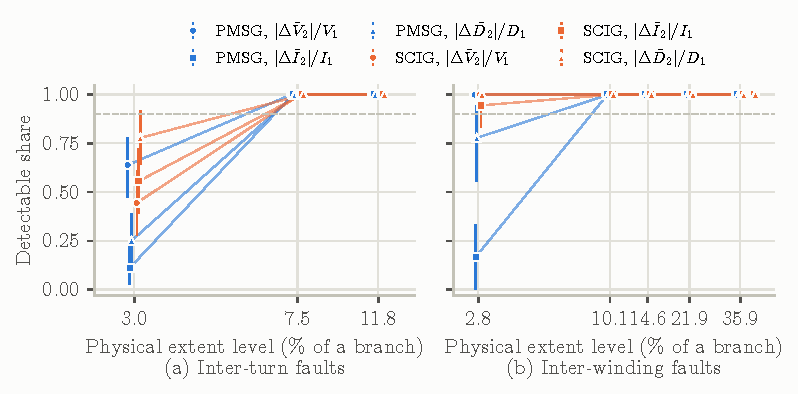
\includegraphics[width=\textwidth]{G_pod}
\caption{Detectable share of the fixed features per physical extent level with 95\,\% bootstrap intervals, PMSG and SCIG, five-cycle windows; dashed, the required power 0.9}\label{fig:pod}
\end{figure*}

The established effect sizes rank the features as the SDR does but set a different threshold. On the same trials, with one AUC per feature from all trials of a class against all healthy changes of the machine, so that each correlation is over the 33 features of one machine and class, the per-feature AUC of the change under fault against the pooled healthy changes ranks the features with a Spearman correlation of 0.94 to 0.99 against the median SDR, the AUC against the nine healthy trials' fault-interval changes with 0.82 to 0.97, and Cohen's $d$ on the drift scale with 0.93 to 0.99; the three top features of each machine and class are shared in two or three cases of three. The threshold is where they can differ, and here they differ little once the reference has the right shape. A parametric rule with a Rayleigh reference for the phasor residuals and a folded-normal reference, $|\delta|\ge1.96\,\sigma_{\delta^0}$, for the scalar features (Fig.~\ref{fig:nullhist}) gives the same MDE as the empirical quantile for 29 to 32 of the 30 to 33 screened features per machine and class (30 on the SCIG, whose shaft-torque features have an unbounded null) and for every residual feature; the empirical quantile lies within 3 to 11\,\% of the parametric one for the fixed features, whereas the scalar reference applied to the residual magnitudes would overstate the difference by a factor of 1.6 to 1.9. What the empirical quantile absorbs is the tail: the excess kurtosis of the residual magnitudes is 1 to 7.5 against 0.25 for a Rayleigh variable, and it varies with speed (0 to 10.5 for the PMSG's voltage residual), as a scale mixture over operating points would produce. The comparison is the one Table~\ref{tab:positioning} predicts: the ranking is a property of the data, the threshold is where the calibration matters, and the added value of the SDR is the calibrated interpretation and the decision organisation built on it, not a different ranking of the informative features.

\begin{figure*}[htbp]
\centering
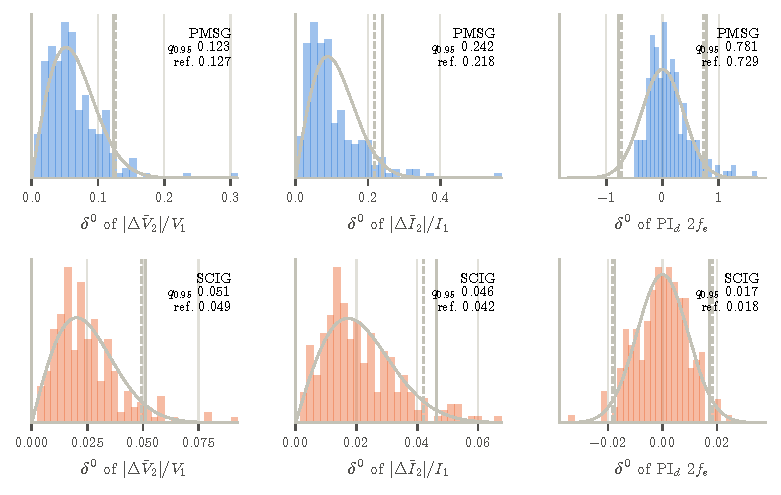
\includegraphics[width=\textwidth]{G_null_hist}
\caption{Drift null of three fixed features, all records, five-cycle windows, with the Rayleigh (residuals) or normal (ripple) density of equal RMS; solid, empirical $q_{0.95}$; dashed, parametric}\label{fig:nullhist}
\end{figure*}

\subsection{Sensor suites and the selection}\label{sec:res-suites}

Table~\ref{tab:suites} gives the suite results for the PMSG and SCIG at five-cycle windows, with the MDE, $e_{90}^{\mathrm{B}}$, the pooled share and the false-alarm count of each fixed feature. For the PMSG, current transducers alone detect inter-turn faults from the middle level and inter-winding faults from 9.7--10.6\,\%. Three voltage transducers take the median criterion to the smallest level for both classes (88 and 100\,\% of trials pooled), but with power 0.9 the inter-turn $e_{90}^{\mathrm{B}}$ stays at the middle level for every suite of both machines. On the six inter-winding levels a log-logistic POD model in extent interpolates between the tested levels: it puts $a_{90}$ at 3.2\,\% (bootstrap 95th percentile 3.7) for the PMSG's duty-cycle residual, 4.5 (4.8) for its current residual and 2.5 (3.1) for the SCIG's, the other fixed features detecting every trial at every level. These sit below the $e_{90}$ and $e_{90}^{\mathrm{B}}$ of the same features because they answer different questions: $a_{90}$ is the point where a fitted curve crosses 0.9 between the smallest level (78\,\% detected for the PMSG's duty-cycle residual) and the next (100\,\%), borrowing the saturated upper levels' strength through the assumed shape, whereas $e_{90}$ reads the first tested level with a share of 0.9 and $e_{90}^{\mathrm{B}}$ the first from which the whole procedure, feature re-selected and null re-estimated, meets it in 95\,\% of resamples. The drive-internal suite reaches the same inter-turn bracket as the current transducers through the duty-cycle residual, and the smallest inter-winding level by the median criterion (96\,\% of trials pooled) but only 14.3--14.8\,\% with power 0.9. For the SCIG the cheapest suites reach what any suite reaches: the smallest level of both classes by the median criterion, through the current residual or, with no added sensor, the duty-cycle residual (93\,\% of inter-turn trials) and the $d$-axis PI output (100\,\% of inter-winding trials); at three cycles every suite stops at the middle level for inter-turn faults. At three cycles the WFSG detects all inter-winding faults from 2.3\,\% with every suite and 92\,\% of the inter-turn trials at the matching impedance, the field current alone 100 and 80\,\%. The fixed features have at most two false alarms in nine healthy trials (Wilson interval 6--55\,\%), a nested selection of the fixed feature on the other tap pairs changes the pooled shares by at most one point at five cycles and six points at three, and the calibrated oracle exceeds the fixed feature's share in one suite only (by three points) and otherwise equals it or falls below it by up to 22 points. Under the tested calibrated maximum statistic, then, the features of a suite buy nothing over its best feature once the false-alarm rate is held; a statistic that sums evidence across features, or a classifier, may still gain, and the window-level detectors of Section~\ref{sec:res-transfer} are the multivariate comparator of this paper. A shaft torque transducer adds nothing for winding faults (median SDR below 0.3 on the PMSG, unbounded null on the SCIG).

%% BEGIN GENERATED tab_suites -- written by scripts/make_tables.py from results/tables; do not edit by hand
\begin{table*}[htbp]
\fontsize{8}{10}\selectfont
\setlength{\tabcolsep}{1.3pt}
\centering
\caption{Sensor suites versus what they detect, PMSG and SCIG, five-cycle windows: fixed feature, MDE bracket, $e_{90}^{\mathrm{B}}$, detectable share and false alarms}\label{tab:suites}
\begin{threeparttable}
\begin{tabular}{@{}lllllllllll@{}}
\toprule
\multirow{2}{*}{Suite} & \multicolumn{5}{c}{PMSG} & \multicolumn{5}{c}{SCIG} \\
\cmidrule(lr){2-6}\cmidrule(l){7-11}
 & feature & MDE & $e_{90}^{\mathrm{B}}$ & DS (or.) & FA & feature & MDE & $e_{90}^{\mathrm{B}}$ & DS (or.) & FA \\
\midrule
\multicolumn{11}{@{}l}{\emph{Inter-turn faults}} \\
drive & $\Delta\bar D_2$ & (3.0,7.5] & 7.5 & 75 (69) & 0/9 & $\Delta\bar D_2$ & $\le$3.0 & 7.5 & 93 (71) & 2/9 \\
3CT & $\Delta\bar I_2$ & (3.0,7.5] & 7.5 & 70 (61) & 0/9 & $\Delta\bar I_2$ & $\le$3.0 & 7.5 & 85 (78) & 1/9 \\
+3VT & $\Delta\bar V_2$ & $\le$3.0 & 7.5 & 88 (75) & 0/9 & $\Delta\bar I_2$ & $\le$3.0 & 7.5 & 85 (77) & 1/9 \\
+drv & $\Delta\bar V_2$ & $\le$3.0 & 7.5 & 88 (69) & 0/9 & $\Delta\bar D_2$ & $\le$3.0 & 7.5 & 93 (74) & 2/9 \\
+torque & $\Delta\bar V_2$ & $\le$3.0 & 7.5$^{\mathrm{a}}$ & 88 (69) & 0/9 & $\Delta\bar D_2$ & $\le$3.0 & 7.5$^{\mathrm{a}}$ & 93 (74) & 2/9 \\
\multicolumn{11}{@{}l}{\emph{Inter-winding faults}} \\
drive & $\Delta\bar D_2$ & $\le$2.8 & 14.6 & 96 (90) & 0/9 & PI$_d$\,2$f_e$ & $\le$2.8 & 2.8 & 100 (100) & 1/9 \\
3CT & $\Delta\bar I_2$ & (2.8,10.1] & 10.1 & 86 (89) & 0/9 & $I_2/I_1$ & $\le$2.8 & 10.1 & 99 (98) & 0/9 \\
+3VT & $\Delta\bar V_2$ & $\le$2.8 & 2.8 & 100 (98) & 0/9 & $V_2/V_1$ & $\le$2.8 & 2.8 & 100 (99) & 0/9 \\
+drv & $\Delta\bar V_2$ & $\le$2.8 & 2.8 & 100 (98) & 0/9 & PI$_d$\,2$f_e$ & $\le$2.8 & 2.8 & 100 (100) & 1/9 \\
+torque & $\Delta\bar V_2$ & $\le$2.8 & 2.8$^{\mathrm{a}}$ & 100 (96) & 0/9 & PI$_d$\,2$f_e$ & $\le$2.8 & 2.8$^{\mathrm{a}}$ & 100 (100) & 1/9 \\
\bottomrule
\end{tabular}
\begin{tablenotes}[flushleft]
\item drive: drive-internal quantities alone; 3CT: three current transducers; +3VT, +drv, +torque: voltage transducers, controller access and a shaft torque transducer added cumulatively to 3CT (each row includes the rows above it from 3CT on). $\Delta\bar X_2$ stands for the residual $|\Delta\bar X_2|/X_1$. MDE: median-crossing extent (Table~\ref{tab:mde}); $e_{90}^{\mathrm{B}}$: smallest tested level (\%) from which the detectable share at the level itself is at least 0.9, at that level and above, with bootstrap support of at least 0.95 (Section~\ref{sec:derived}; not a confidence bound). DS (\%) of the fixed feature pooled over all tested extents, in parentheses the share of the calibrated oracle (Section~\ref{sec:sdr}); the nested selection of the fixed feature on the other tap pairs changes these shares by at most one point at this window length (Table~\ref{tab:heldout} gives the held-out run of the whole procedure). FA: false alarms of the fixed feature on the nine healthy trials; screened-out features are excluded.
\item[a] Same fixed feature as +drv; the torque features add nothing.
\end{tablenotes}
\end{threeparttable}
\end{table*}
%% END GENERATED tab_suites

The decision table (Table~\ref{tab:decision}) turns this into the selection of step~5, with the power required at the level itself. For inter-turn faults at the smallest level (2.7--3.8\,\% of a branch) every suite on both machines fails: the fixed features detect 11 to 78\,\% of the trials at that level, and the resampling support for a share of 0.9 is at most 0.04 (the two SCIG cells nearest the boundary read 0.036 and 0.049 at 1000 resamples, 0.040 at 10\,000, and 0.002 under tap-pair resampling; no cell of Table~\ref{tab:decision} lies within two Monte-Carlo standard errors of a boundary at 10\,000 resamples). From the middle level (7.4--7.7\,\%) every suite on both machines meets the requirement with support of at least 0.99; on the WFSG only the largest level is testable at the matching impedance, and there every suite meets it except the field current alone (0.92). For inter-winding faults the SCIG meets the requirement at the smallest level with the drive-internal suite and with every suite that holds voltage transducers, its current transducers alone being uncertain there (0.75, with 94\,\% of that level's trials detected) and adequate from 9.7--10.6\,\%; the WFSG meets it at both of its testable levels with every suite. The PMSG meets it at the smallest level only with voltage transducers: its current transducers fail there and meet from 9.7--10.6\,\%, and its drive-internal suite is uncertain at the smallest level (0.10, 78\,\% detected) and at 9.7--10.6\,\% (0.88, every trial detected but the null and the feature re-estimated) and meets from 14.3--14.8\,\%. Relaxing $\alpha$ to 0.90 or tightening it to 0.99 changes no verdict at the level itself except the PMSG's current-only suite at the middle inter-turn level, which becomes uncertain at 0.99 (0.53); on three-cycle windows the SCIG's inter-turn verdicts at the smallest level fail for every suite (Section~\ref{sec:res-robust}).

%% BEGIN GENERATED tab_decision -- written by scripts/make_tables.py from results/tables; do not edit by hand
\begin{table*}[htbp]
\tabsize
\setlength{\tabcolsep}{2.6pt}
\centering
\caption{Decision table at $\alpha=0.95$: bootstrap support for a suite meeting the empirical requirement at each tested extent level}\label{tab:decision}
\begin{threeparttable}
\begin{tabular}{@{}lcccccccccccc@{}}
\toprule
Suite & \multicolumn{4}{c}{PMSG} & \multicolumn{4}{c}{SCIG} & \multicolumn{4}{c}{\shortstack{WFSG\\(exploratory, unscreened)}} \\
\cmidrule(lr){2-5}\cmidrule(lr){6-9}\cmidrule(l){10-13}
 & \multicolumn{12}{c}{bootstrap support for meeting the empirical requirement at $e_{\mathrm{req}}$} \\
\midrule
\multicolumn{13}{@{}l}{\emph{Inter-turn faults}} \\
$e_{\mathrm{req}}$ (\%) & 3.0 & 7.5 & 11.8 &  & 3.0 & 7.5 & 11.8 &  & 3.0 & 7.5 & 11.8 & \\
drive & 0.00 & \textbf{1.00} & \textbf{1.00} &  & 0.04 & \textbf{1.00} & \textbf{1.00} &  & n.t. & n.t. & \textbf{1.00} & \\
3CT & 0.00 & \textbf{0.99} & \textbf{1.00} &  & 0.00 & \textbf{1.00} & \textbf{1.00} &  & n.t. & n.t. & \textbf{1.00} & \\
3CT+3VT & 0.00 & \textbf{1.00} & \textbf{1.00} &  & 0.00 & \textbf{1.00} & \textbf{1.00} &  & n.t. & n.t. & \textbf{1.00} & \\
3CT+3VT+drv & 0.00 & \textbf{1.00} & \textbf{1.00} &  & 0.04 & \textbf{1.00} & \textbf{1.00} &  & n.t. & n.t. & \textbf{1.00} & \\
exc & -- & -- & -- &  & -- & -- & -- &  & n.t. & n.t. & 0.92 & \\
\multicolumn{13}{@{}l}{\emph{Inter-winding faults}} \\
$e_{\mathrm{req}}$ (\%) & 2.8 & 10.1 & 14.6 & 21.9 & 2.8 & 10.1 & 14.6 & 21.9 & 2.8 & 10.1 & 14.6 & 21.9 \\
drive & 0.10 & 0.88 & \textbf{1.00} & \textbf{1.00} & \textbf{1.00} & \textbf{1.00} & \textbf{1.00} & \textbf{1.00} & \textbf{1.00} & \textbf{1.00} & n.t. & n.t. \\
3CT & 0.00 & \textbf{0.97} & \textbf{0.98} & \textbf{0.98} & 0.75 & \textbf{1.00} & \textbf{1.00} & \textbf{1.00} & \textbf{1.00} & \textbf{1.00} & n.t. & n.t. \\
3CT+3VT & \textbf{1.00} & \textbf{1.00} & \textbf{1.00} & \textbf{1.00} & \textbf{1.00} & \textbf{1.00} & \textbf{1.00} & \textbf{1.00} & \textbf{1.00} & \textbf{1.00} & n.t. & n.t. \\
3CT+3VT+drv & \textbf{1.00} & \textbf{1.00} & \textbf{1.00} & \textbf{1.00} & \textbf{1.00} & \textbf{1.00} & \textbf{1.00} & \textbf{1.00} & \textbf{1.00} & \textbf{1.00} & n.t. & n.t. \\
exc & -- & -- & -- & -- & -- & -- & -- & -- & \textbf{1.00} & \textbf{1.00} & n.t. & n.t. \\
\bottomrule
\end{tabular}
\begin{tablenotes}[flushleft]
\item Cell: fraction of resamples (10\,000 for the PMSG and SCIG, 1000 for the WFSG) in which $\mathrm{MDE}\le e_{\mathrm{req}}$ and the detectable share at the tested level that $e_{\mathrm{req}}$ maps to is $\ge0.9$; resampling support, an empirical stability measure of the decision, not a posterior probability and not a confidence level; a cell of 1.00 means no resample failed. $e_{\mathrm{req}}$ at the physical levels of the common bench (\% of a branch; the WFSG, unscreened for lack of healthy trials, is assessed against the same values on its own tested extents); the operating-point trials of a level are resampled with its tap pairs treated as exchangeable, null quantile and fixed feature re-estimated in every resample. Bold: support $\ge0.95$ (meets); $\le0.05$: fails; between: uncertain; n.t.: no tested extent on the required side of $e_{\mathrm{req}}$. PMSG and SCIG at five-cycle windows, WFSG at three cycles and its matching fault impedance; the inter-winding levels 35.9 and 40.2\,\% are omitted (every suite meets them). Suites as in Table~\ref{tab:suites}; exc: WFSG field current. Table~\ref{tab:cells} gives the cells that change under the pooled share or the tap-pair resampling unit.
\end{tablenotes}
\end{threeparttable}
\end{table*}
%% END GENERATED tab_decision

Table~\ref{tab:cells} lists the eight cells whose verdict depends on the definition of the power or on the resampling unit; every other cell of Table~\ref{tab:decision}, the WFSG's included, keeps its verdict under all four variants. Pooling the share over all tested extents above the requirement, as a bench's mix of extents would, raises four failing inter-turn cells to uncertain (0.27 for the PMSG's voltage suite, 0.82 for the SCIG's drive-internal suite) and two uncertain inter-winding cells to meets, because the larger faults, which outnumber the smallest level, are all detected. Resampling tap pairs instead of trials moves the cells by at most 0.10 and changes one verdict, the PMSG's drive-internal suite at the smallest inter-winding level, from uncertain (0.10) to fails (0.00).

Table~\ref{tab:heldout} reports the held-out run of the complete procedure. For each tap pair in turn the pooled null quantile, the screen and the fixed feature of every suite are fitted on the other tap pairs and the healthy trials, frozen, and applied to the held-out pair, whose trials keep their own pre-fault reference. The held-out $e_{90}$ equals the in-sample one for all sixteen suite--class pairs; the held-out share at the smallest level differs from the in-sample one in two cells by at most six points (the PMSG's drive-internal suite 83 against 78\,\% and the SCIG's voltage suite 94 against 100\,\% for inter-winding faults); and the folds choose the in-sample feature or one equivalent to it. The frozen procedure's false alarms, each healthy trial held out of the null and the selection in turn, are 0 of 9 on the PMSG and 1 to 3 of 9 on the SCIG, against 0 and 1 to 2 in sample; the 3 of 9 belong to the $d$-axis PI ripple, the in-sample fixed feature of the inter-winding drive-internal suite (1 of 9 in sample; the $d$-axis current ripple and the duty-cycle residual tie with it on extent and share, and the folds choose among the three), a count the screen would reject, so that cell's false-alarm rate is the least secure in Table~\ref{tab:decision}. Selecting the feature by the share at the required level instead of by the MDE, inside every resample, changes one cell: the PMSG's drive-internal suite at 9.7--10.6\,\% for inter-winding faults moves from uncertain (0.88) to meets (1.00); every other verdict stands, so the verdicts are, with that exception, also those of the best feature at the requirement.

%% BEGIN GENERATED tab_heldout -- written by scripts/make_tables.py from results/tables; do not edit by hand
\begin{table*}[htbp]
\tabsize
\setlength{\tabcolsep}{3pt}
\centering
\caption{Held-out run of the complete procedure, PMSG and SCIG, five-cycle windows: fixed feature, $e_{90}$ and share at the smallest level, in sample / held out, and false alarms of the frozen procedure}\label{tab:heldout}
\begin{threeparttable}
\begin{tabular}{@{}lllllllll@{}}
\toprule
\multirow{2}{*}{Suite} & \multicolumn{4}{c}{PMSG} & \multicolumn{4}{c}{SCIG} \\
\cmidrule(lr){2-5}\cmidrule(l){6-9}
 & feature & $e_{90}$ in/out & share in/out & FA & feature & $e_{90}$ in/out & share in/out & FA \\
\midrule
\multicolumn{9}{@{}l}{\emph{Inter-turn faults}} \\
drive & $\Delta\bar D_2$ & 7.5 / 7.5 & 25 / 25 & 0/9 & $\Delta\bar D_2$ & 7.5 / 7.5 & 78 / 78 & 2/9 \\
3CT & $\Delta\bar I_2$ & 7.5 / 7.5 & 11 / 11 & 0/9 & $\Delta\bar I_2$ & 7.5 / 7.5 & 56 / 56 & 1/9 \\
3CT+3VT & $\Delta\bar V_2$ & 7.5 / 7.5 & 64 / 64 & 0/9 & $\Delta\bar I_2$ & 7.5 / 7.5 & 56 / 56 & 1/9 \\
3CT+3VT+drv & $\Delta\bar V_2$ & 7.5 / 7.5 & 64 / 64 & 0/9 & $\Delta\bar D_2$ & 7.5 / 7.5 & 78 / 78 & 2/9 \\
\multicolumn{9}{@{}l}{\emph{Inter-winding faults}} \\
drive & $\Delta\bar D_2$ & 10.1 / 10.1 & 78 / 83 & 0/9 & PI$_d$\,2$f_e$$^{\mathrm{a}}$ & 2.8 / 2.8 & 100 / 100 & 3/9 \\
3CT & $\Delta\bar I_2$ & 10.1 / 10.1 & 17 / 17 & 0/9 & $I_2/I_1$$^{\mathrm{b}}$ & 2.8 / 2.8 & 94 / 94 & 0/9 \\
3CT+3VT & $\Delta\bar V_2$ & 2.8 / 2.8 & 100 / 100 & 0/9 & $V_2/V_1$$^{\mathrm{c}}$ & 2.8 / 2.8 & 100 / 94 & 0/9 \\
3CT+3VT+drv & $\Delta\bar V_2$ & 2.8 / 2.8 & 100 / 100 & 0/9 & PI$_d$\,2$f_e$$^{\mathrm{d}}$ & 2.8 / 2.8 & 100 / 100 & 3/9 \\
\bottomrule
\end{tabular}
\begin{tablenotes}[flushleft]
\item Held out: for each tap pair in turn, the pooled null quantile, the screen and the suite's fixed feature are fitted on the records of the other tap pairs and the healthy trials, frozen, and applied to the held-out pair's nine trials, which keep their own pre-fault reference; shares aggregate the held-out trials by physical level. Feature: in-sample fixed feature; a letter marks a suite whose folds chose another feature as well. $e_{90}$ (\%): smallest tested level from which the share at the level is $\ge0.9$ at every level up; -- when none. Share (\%) at the smallest tested level of the class. FA: false alarms of the frozen procedure on the nine healthy trials, each held out of the null and the selection in turn.
\item[a] Some folds chose $\Delta\bar D_2$ or $I_d$\,2$f_e$ instead.
\item[b] Some folds chose $\Delta\bar I_2$ instead.
\item[c] Some folds chose $I_2/I_1$ or $\Delta\bar I_2$ instead.
\item[d] Some folds chose $\Delta\bar D_2$ or $I_d$\,2$f_e$ instead.
\end{tablenotes}
\end{threeparttable}
\end{table*}
%% END GENERATED tab_heldout

%% BEGIN GENERATED tab_cells -- written by scripts/make_tables.py from results/tables; do not edit by hand
\begin{table*}[htbp]
\tabsize
\setlength{\tabcolsep}{4pt}
\centering
\caption{Decision-table cells whose verdict depends on the definition of the power or on the resampling unit within a level, or lies at a boundary}\label{tab:cells}
\begin{threeparttable}
\begin{tabular}{@{}lllcccccc@{}}
\toprule
\multirow{2}{*}{Machine} & \multirow{2}{*}{Class} & \multirow{2}{*}{Suite} & \multirow{2}{*}{$e_{\mathrm{req}}$ (\%)} & \multirow{2}{*}{DS at level} & \multicolumn{2}{c}{at level} & \multicolumn{2}{c}{pooled} \\
\cmidrule(lr){6-7}\cmidrule(l){8-9}
 & & & & & trials & pairs & trials & pairs \\
\midrule
PMSG & inter-turn & 3CT+3VT & 3.0 & 64 & 0.00 & 0.01 & 0.27 & 0.23 \\
PMSG & inter-turn & 3CT+3VT+drv & 3.0 & 64 & 0.00 & 0.01 & 0.27 & 0.23 \\
PMSG & inter-winding & drive & 2.8 & 78 & 0.10 & 0.00 & 0.93 & 0.93 \\
PMSG & inter-winding & drive & 10.1 & 100 & 0.88 & 0.94 & 1.00 & 1.00 \\
SCIG & inter-turn & drive & 3.0 & 78 & 0.04 & 0.00 & 0.82 & 0.89 \\
SCIG & inter-turn & 3CT+3VT & 3.0 & 56 & 0.00 & 0.00 & 0.052 & 0.00 \\
SCIG & inter-turn & 3CT+3VT+drv & 3.0 & 78 & 0.04 & 0.00 & 0.82 & 0.92 \\
SCIG & inter-winding & 3CT & 2.8 & 94 & 0.75 & 0.71 & 1.00 & 1.00 \\
\bottomrule
\end{tabular}
\begin{tablenotes}[flushleft]
\item $\alpha=0.95$; every other cell of Table~\ref{tab:decision} keeps its verdict under all four variants. At level, trials: 10\,000 resamples (Table~\ref{tab:decision}); the other three variants 1000. DS at level: share of the fixed feature at the level $e_{\mathrm{req}}$ maps to (\%). At level: share at that level (Table~\ref{tab:decision}); pooled: share over all tested levels $\ge e_{\mathrm{req}}$; trials, pairs: resampling unit within a level. Meets at $\ge0.95$, fails at $\le0.05$, classified on the unrounded fraction.
\end{tablenotes}
\end{threeparttable}
\end{table*}
%% END GENERATED tab_cells

\subsection{Transfer across machines}\label{sec:res-transfer}

Table~\ref{tab:transfer} reports step~6 for the PMSG--SCIG pair on five-cycle windows: the GBDT detector on the out-of-reference windows, with 95\,\% cluster-bootstrap intervals and the true-positive rate (TPR) at 1\,\% false-positive rate. In physical units the detector reaches an AUC of 0.93 and 0.91 within a machine on unseen tap pairs but 0.79 [0.68, 0.88] (PMSG$\to$SCIG) and 0.61 [0.50, 0.72] (SCIG$\to$PMSG) across, with a TPR of 0.25 and 0.26 across against 0.74 and 0.67 within. Any referencing to healthy behaviour of the target machine recovers most of the AUC, the self-referenced rule reaching 0.93 [0.87, 0.98] and 0.89 [0.82, 0.95] against 0.87--0.88 for the two commissioning baselines. The rules separate on the TPR, where the self-referenced rule gives 0.81 [0.67, 0.94] and 0.54 [0.37, 0.69] against 0.50--0.71 and 0.54--0.62 for the baselines, and on the linear detector, a logistic regression transferring at 0.93 and 0.91 when self-referenced but at 0.49--0.81 under the baselines. The self-referenced rule is thus the best on AUC in both directions and on TPR in one, with overlapping intervals in the other, and the ranking of the rules is the result of interest: self-referencing turns a classifier into a change detector, so that it transfers is less surprising than how much the other rules lose. Between the three machines, on three-cycle windows, self-referenced GBDT detectors transfer in all six directions with an AUC of 0.85 [0.79, 0.91] to 0.98 [0.96, 1.00] and a TPR of 0.41 to 0.94, against 0.90--0.97 and 0.71--0.93 within a machine, and a detector trained on two machines detects the faults of the third with an AUC of 0.87 (PMSG), 0.90 (SCIG) and 0.99 (WFSG; optimistic, as that bench has no healthy trials). These are results for abrupt-onset detection against a stationary healthy background: the negatives hold the contactor operation and the release transient but no load change, speed ramp or grid disturbance, and a TPR of 0.54 at 1\,\% false positives in one direction is not a field-ready detector.

%% BEGIN GENERATED tab_transfer -- written by scripts/make_tables.py from results/tables; do not edit by hand
\begin{table*}[htbp]
\fontsize{8}{10}\selectfont
\setlength{\tabcolsep}{2pt}
\centering
\caption{GBDT detector transferred between PMSG and SCIG under four referencing rules, out-of-reference windows}\label{tab:transfer}
\begin{threeparttable}
\begin{tabular}{@{}llC{2.05cm}C{2.05cm}C{2.05cm}C{2.05cm}@{}}
\toprule
Direction & Metric & physical units & $z$, all healthy trials of the target & $z$, healthy trial at the operating point & $|z|$ against own reference \\
\midrule
P$\to$P & AUC & 0.93 [0.86, 0.98] & 0.93 [0.86, 0.98] & 0.91 [0.84, 0.96] & 0.94 [0.90, 0.98] \\
 & TPR & 0.74 [0.55, 0.89] & 0.74 [0.55, 0.89] & 0.63 [0.43, 0.83] & 0.78 [0.64, 0.91] \\
S$\to$S & AUC & 0.91 [0.83, 0.97] & 0.91 [0.83, 0.97] & 0.91 [0.84, 0.96] & 0.96 [0.92, 0.99] \\
 & TPR & 0.67 [0.50, 0.85] & 0.67 [0.50, 0.85] & 0.62 [0.43, 0.79] & 0.82 [0.68, 0.94] \\
P$\to$S & AUC & 0.79 [0.68, 0.88] & 0.88 [0.81, 0.95] & 0.87 [0.79, 0.95] & 0.93 [0.87, 0.98] \\
 & TPR & 0.25 [0.14, 0.35] & 0.50 [0.36, 0.67] & 0.71 [0.57, 0.87] & 0.81 [0.67, 0.94] \\
S$\to$P & AUC & 0.61 [0.50, 0.72] & 0.88 [0.81, 0.94] & 0.88 [0.80, 0.94] & 0.89 [0.82, 0.95] \\
 & TPR & 0.26 [0.10, 0.40] & 0.54 [0.32, 0.71] & 0.62 [0.42, 0.76] & 0.54 [0.37, 0.69] \\
\bottomrule
\end{tabular}
\begin{tablenotes}[flushleft]
\item AUC and true-positive rate at 1\,\% false-positive rate (TPR) on the out-of-reference windows (Section~\ref{sec:computation}); intervals from 500 cluster resamples of the tested machine's trials. P$\to$P, S$\to$S: cross-validation grouped by tap pair; P$\to$S, S$\to$P: trained on one machine, tested on the other.
\end{tablenotes}
\end{threeparttable}
\end{table*}
%% END GENERATED tab_transfer

\subsection{Operating envelope, conventions and the two nulls}\label{sec:res-robust}\label{sec:res-op}

Table~\ref{tab:envelope} gives the operating envelope. Speed dominates: between 1200 and 1800\,rpm the median inter-turn SDR of the fixed features of Table~\ref{tab:suites} rises by a factor of 1.3 to 4.4 and the pooled shares from 69--86 to 83--100\,\%, consistent with a resistor-limited fault current that scales with speed. Torque changes the medians at a fixed speed by less than a factor 1.25 on the SCIG and up to 1.6 on the PMSG. The PMSG's current residual, the feature of its retrofit suite, is the exception, falling from 1.8 to 1.4 with speed with its share fixed at 67\,\%. The terminal impedance $|\Delta\bar V_2/\Delta\bar I_2|$ does not explain that exception: it is flat within 5\,\% over $2f_e$ = 80 to 120\,Hz on both machines (13.0 to 12.5\,$\Omega$ on the PMSG, 7.5 to 7.2\,$\Omega$ on the SCIG), so it is not proportional to frequency as a leakage reactance would be, and the bandwidth mechanism of Section~\ref{sec:implications} is not visible inside this band. Because the pooled null is a mixture over operating points, the 5\,\% false-alarm reading holds on average over the envelope. The share of healthy changes above the pooled 95th percentile is 0 to 16\,\% by speed for the key features, the largest being the SCIG's current residual at 1800\,rpm, where its null quantile is 1.7 times the one at 1200\,rpm. The proximity of its 59.6\,Hz electrical frequency to the 60\,Hz grid frequency was tested as a cause on the raw healthy records: a joint least-squares fit of the stator current to the fundamental and a grid-frequency component finds a second tone of 2 to 4\,\% of the fundamental at 1800\,rpm, but a tone 0.25 to 0.6\,Hz from the fundamental fits 1 to 4\,\% at 1200 and 1500\,rpm as well, where a 60\,Hz component itself is below 0.1\,\%; the tone is a slow modulation of the fundamental present at every speed, and the wider null at 1800\,rpm remains unexplained. A null quantile estimated per speed (75 records each; Table~\ref{tab:conventions}) changes the MDE of two of the twelve key feature--class pairs, moving the SCIG's voltage residual down to the smallest inter-turn level and the PMSG's $q$-axis ripple to the middle one, and leaves the verdicts of Table~\ref{tab:decision} unchanged. At the lowest speed the smallest inter-turn level is detected in 8 to 50\,\% of the trials by the fixed features, so a requirement written at every operating point fails there as the pooled one does, and the lowest monitored speed is a parameter of the requirement.

%% BEGIN GENERATED tab_envelope -- written by scripts/make_tables.py from results/tables; do not edit by hand
\begin{table*}[htbp]
\tabsize
\setlength{\tabcolsep}{3pt}
\centering
\caption{Operating envelope: fixed inter-turn features and terminal impedance by speed, PMSG and SCIG, five-cycle windows}\label{tab:envelope}
\begin{threeparttable}
\begin{tabular}{@{}llcccc@{}}
\toprule
Machine & Feature / class & 1200\,rpm & 1500\,rpm & 1800\,rpm & Torque factor \\
\midrule
\multicolumn{6}{@{}l}{\emph{Median SDR (detectable share, \%) of the fixed inter-turn features}} \\
PMSG & $|\Delta\bar V_2|/V_1$ & 5.3 (78) & 7.0 (89) & 10.0 (97) & 1.36 \\
PMSG & $|\Delta\bar D_2|/D_1$ & 2.7 (69) & 4.0 (72) & 5.6 (83) & 1.64 \\
PMSG & $|\Delta\bar I_2|/I_1$ & 1.8 (67) & 2.6 (78) & 1.4 (67) & 1.59 \\
SCIG & $|\Delta\bar I_2|/I_1$ & 3.8 (69) & 6.3 (86) & 16.6 (100) & 1.21 \\
SCIG & $|\Delta\bar D_2|/D_1$ & 9.5 (86) & 11.6 (94) & 12.2 (97) & 1.18 \\
SCIG & $|\Delta\bar V_2|/V_1$ & 5.8 (78) & 7.3 (83) & 8.2 (83) & 1.15 \\
\multicolumn{6}{@{}l}{\emph{Incremental negative-sequence impedance $|\Delta\bar V_2/\Delta\bar I_2|$ ($\Omega$), median [IQR]}} \\
PMSG & inter-turn & 13.0 [11.5, 14.4] & 12.6 [11.3, 14.1] & 12.5 [10.0, 13.8] & \\
PMSG & inter-winding & 12.6 [11.1, 13.3] & 12.1 [9.2, 13.7] & 11.9 [9.8, 12.8] & \\
SCIG & inter-turn & 7.5 [7.0, 8.0] & 7.2 [6.7, 7.4] & 7.2 [6.9, 7.4] & \\
SCIG & inter-winding & 7.5 [7.4, 7.8] & 7.4 [7.3, 7.6] & 7.3 [7.1, 7.4] & \\
\bottomrule
\end{tabular}
\begin{tablenotes}[flushleft]
\item Speeds 1200, 1500 and 1800\,rpm ($2f_e$ = 80, 100 and 120\,Hz; 79, 99 and 119\,Hz on the SCIG, which generates with slip); each cell pools the three torques (36 inter-turn trials per machine and speed). Torque factor: largest ratio of per-torque medians at a fixed speed. The impedance is the per-trial complex ratio of the phasor residuals (Section~\ref{sec:res-where}), 36 trials per cell.
\end{tablenotes}
\end{threeparttable}
\end{table*}
%% END GENERATED tab_envelope

Table~\ref{tab:conventions} also gives the interval and reference conventions. Starting the faulted interval 120\,ms after the command, after the relay has picked up, raises the median SDR of the fixed inter-turn features by 6 to 8\,\% and changes no MDE, so the 55\,ms of healthy time in the baseline interval dilutes the signature slightly and adds no transient. Recomputing the common-bench SDRs with the WFSG's geometry, a 150\,ms faulted interval and 190\,ms reference halves, lowers the medians by up to 36\,\% (the voltage residuals most, the current residuals by 8\,\% or less), widens the null and moves the MDE of the PMSG's voltage residual and the SCIG's current residual up one level; the ordering of the two machines is unchanged. The WFSG's shorter intervals therefore penalise it rather than favour it, and its SDRs in Fig.~\ref{fig:features} are conservative on that account. Pooling the WFSG over its fault impedances lowers its inter-turn medians relative to the 2.83\,$\Omega$ subset (10.9 against 16.1 for the voltage residual) and raises its inter-winding ones (35 against 14), because the large-extent inter-winding pairs were tested at the highest resistances. The negative-sequence estimate itself is not limited by the short windows: on a synthetic three-phase signal with the PMSG's inherent asymmetry ($I_2/I_1 = 0.006$) a three-cycle Hann window recovers the ratio within 0.2\,\%, and within 1.6\,\% when the electrical frequency used is 1\,\% wrong.

%% BEGIN GENERATED tab_conventions -- written by scripts/make_tables.py from results/tables; do not edit by hand
\begin{table*}[htbp]
\tabsize
\setlength{\tabcolsep}{3pt}
\centering
\caption{Detectable share (\%) and MDE of the fixed inter-turn features under other interval, null and reference conventions, five-cycle windows}\label{tab:conventions}
\begin{threeparttable}
\begin{tabular}{@{}L{4.8cm}cccccc@{}}
\toprule
\multirow{2}{*}{Convention} & \multicolumn{3}{c}{PMSG} & \multicolumn{3}{c}{SCIG} \\
\cmidrule(lr){2-4}\cmidrule(l){5-7}
 & $\Delta\bar V_2$ & $\Delta\bar D_2$ & $\Delta\bar I_2$ & $\Delta\bar I_2$ & $\Delta\bar D_2$ & $\Delta\bar V_2$ \\
\midrule
Baseline (Section~\ref{sec:computation}) & 88 (3.0) & 75 (7.5) & 70 (7.5) & 85 (3.0) & 93 (3.0) & 81 (7.5) \\
Fault interval from 120\,ms after the command & 89 (3.0) & 76 (7.5) & 71 (7.5) & 86 (3.0) & 94 (3.0) & 82 (7.5) \\
WFSG geometry: 150\,ms fault, 190\,ms reference halves & 79 (7.5) & 72 (7.5) & 69 (7.5) & 83 (7.5) & 90 (3.0) & 68 (7.5) \\
Null quantile per speed (75 records each) & 89 (3.0) & 78 (7.5) & 70 (7.5) & 90 (3.0) & 93 (3.0) & 85 (3.0) \\
Reference: healthy trial at the same operating point & 72 (7.5) & 71 (7.5) & 49 (11.8) & 69 (7.5) & 68 (7.5) & 67 (7.5) \\
\bottomrule
\end{tabular}
\begin{tablenotes}[flushleft]
\item $\Delta\bar X_2$ stands for the residual $|\Delta\bar X_2|/X_1$. Cells: detectable share over the 108 inter-turn trials (MDE, \% of a branch; --: largest level not detected). The stricter start excludes the relay pick-up; the WFSG geometry shortens the faulted interval and the reference halves to those of the WFSG bench; the per-speed null replaces the pooled 95th percentile by one per speed; the last row replaces the trial's own reference by the healthy trial recorded at the same operating point at another time (Section~\ref{sec:res-robust}).
\end{tablenotes}
\end{threeparttable}
\end{table*}
%% END GENERATED tab_conventions

With the screen applied at every setting, the MDE brackets of the key features are unchanged across window lengths of three, five and eight cycles on both machines except at the margin (the SCIG's current residual reaches the smallest inter-turn level at five and eight cycles but not at three; the PMSG's $q$-axis voltage ripple reaches the middle level only at eight cycles; the PMSG's $d$-axis features, whose null quantile exceeds one at eight cycles, are screened out there), and the pooled shares move by at most 7 points except for the PMSG's $d$-axis features, which lie below $\mathrm{SDR}=1$ at every setting. Tightening $\alpha$ from 0.95 to 0.99 lowers the shares by 0 to 14 points, moves the MDE up one level for the PMSG's voltage residual and the SCIG's current residual and screens out the PMSG's $d$-axis features; relaxing it to 0.90 raises the shares by up to 10 points and moves four MDEs down one level; the orderings of the two machines are the same at every setting. At $\alpha=0.95$ the screen removes only the SCIG's duty-cycle magnitude ratio (three false alarms in nine healthy trials) and the torque features. An absolute-change variant of the SDR, which divides neither change by the healthy level, ranks the 33 features with a Spearman correlation of 0.92--0.99 against the relative variant and changes the SDR of the residual features by 2 to 56\,\%, but no MDE and no $e_{90}$ of the sixteen suite--class pairs, and no fixed feature except one, where two equivalent magnitude ratios swap.

Replacing the reference immediately before the fault by the healthy trial recorded at the same operating point at another time, a commissioning baseline, widens the null of the four key features by a factor of 1.1 to 4.5 (1.9 to 3.2 for the voltage and current residuals). It lowers the median SDR of the inter-turn residuals from 6.8 to 2.4 (PMSG, voltage) and from 6.3 to 2.1 (SCIG, current), their pooled shares from 88 and 85\,\% to 72 and 69\,\%, and moves the inter-turn MDE up one level for the PMSG's voltage residual and the SCIG's current and duty-cycle residuals and the inter-winding MDE of the SCIG's current and controller features from the smallest level to 9.7--10.6\,\% (Table~\ref{tab:conventions}), while inter-winding faults remain detectable in 67--93\,\% of trials. The two reference ages tested, the preceding half second and the session, bracket the horizon a field monitor must choose.
%% ----------------------------------------------------------------------
%% discussion
%% ----------------------------------------------------------------------

\section{Discussion}\label{sec:discussion}

\subsection{What the demonstration establishes about the method}

The demonstration supports four claims about the method and corrects the naive form of three of them. \emph{The design-level description of a failure mode does not fix its physical severity, and a test matrix can carry a hidden variable.} The same winding fraction produced fault currents differing by a factor of 2.3 relative to the stator current between the PMSG and the SCIG. The faulted phase rode on the nominal extent axis, which the phasor residuals remove and the magnitude ratios do not. A comparison of candidates must therefore carry a severity covariate beside the design extent and use features invariant to the nuisance variables of the matrix. \emph{Where a failure becomes observable is a property of the machine--drive combination, to be read with the decomposition in both forms.} ``The control structure decides'' is not supported, since both machines run the same controller and are indistinguishable through the voltage residual. ``The SCIG wins only by a quieter null'' holds for the stator current but not for the controller quantities. A design team must know whether a candidate wins by signature or by silence, because a signature belongs to the fault physics and a null to the sensing and control chain, which the design-stage outlook of Section~\ref{sec:scope} could not simulate. \emph{The cheapest adequate sensor suite depends on the candidate and on the requirement, and here it changes the monitoring specification, not the choice of machine.} With power 0.9 at the level, the smallest inter-turn level is met by no suite on either machine of the common bench and the middle level by every suite, drive-internal quantities included; at the smallest inter-winding level the PMSG alone needs voltage transducers. \emph{A monitoring design transfers across candidates under a healthy-referenced rule, which belongs in the specification.} Every healthy-referenced rule recovered most of the AUC lost in physical units and the self-referenced rule the most, in both directions and across all three machines. The rules differ in the true-positive rate and for the linear detector, so the stronger claim that a detector transfers \emph{only} when self-referenced is not supported. A specification should name the referencing rule and the horizon over which the reference is renewed, since the self-referenced rule is an abrupt-onset detector that a slowly growing fault would evade.

\subsection{Implications for the condition monitoring of wind-turbine generators}\label{sec:implications}

Within the scope of Section~\ref{sec:threats}, the implications are conditional on the tested machines, the assumed cost ordering and the requirement. A PMSG with full-power conversion should be specified with terminal voltage measurement, or with another observable of the terminal asymmetry such as the zero-sequence voltage where a neutral is accessible \citep{Urresty2012}, if inter-winding faults of the smallest tested size (2.3--3.2\,\% of a branch) are to be detected by threshold monitoring with power 0.9. For inter-turn faults the voltage measurement raises the share of detected trials at the smallest level from 11--25 to 64\,\% without making that level a confident requirement, and from the middle level the controller's duty-cycle residual suffices. An SCIG reaches the same detectability with no added sensor through its controller quantities, but for inter-winding faults that drive-internal suite meets the empirical detection-power criterion with a false-alarm performance that the held-out run leaves to be validated (Table~\ref{tab:heldout}), so it is a candidate specification, not a validated one; with current transducers alone the smallest inter-winding level is uncertain. A third-party retrofit limited to current and voltage transducers reads Table~\ref{tab:decision} as follows. On the PMSG, three current transducers meet the requirement from the middle inter-turn level and from 9.7--10.6\,\% for inter-winding faults, voltage transducers are needed at the smallest inter-winding level, and nothing meets the smallest inter-turn level. On the SCIG, three current transducers meet inter-turn faults from the middle level and inter-winding faults from 9.7--10.6\,\%, the smallest level being uncertain. The least-cost adequate suite is therefore the least-cost one among the specified candidates under the stated ordering, and the ordering of a converter manufacturer and of a retrofit provider give different answers for the SCIG's inter-winding faults. A wound-field machine with a static exciter offers the field current as a further drive-internal channel, whose 2$f_e$ ripple detected every inter-winding fault and 80\,\% of the inter-turn trials at the matching impedance; a brushless exciter would not expose it \citep{Neti2009}.

In the field the null is the quantity a practitioner must establish, and three choices follow from the results. The reference horizon: the SDR as defined uses the half second before the decision, which a rolling reference renews continuously and which a slowly growing fault would enter; a commissioning baseline recorded once widens the null by a factor of 1.1 to 4.5 here and moves the inter-turn MDEs up one level (Section~\ref{sec:res-robust}). A monitor should therefore keep two references, a rolling one for abrupt changes and a frozen one for slow growth, and the specification should name both horizons. The operating-point dependence: a wind turbine moves through its envelope continuously, so the null must be estimated per operating region, as the per-speed null of Table~\ref{tab:conventions} does on the bench, or the operating point must be regressed out of the feature as novelty detection under environmental and operational variability does \citep{Sohn2007, Cross2011}; with 75 records per speed the per-speed null changed two MDEs here, and a field baseline will need weeks of healthy operation to cover the envelope with that density. The decision rate: $\alpha=0.95$ is a false alarm every 7\,s at one decision per interval, so a field monitor needs an accumulation rule, for instance a run of exceedances or a CUSUM on the SDR, and the per-decision rate of the specification should be derived from the tolerated alarm rate per month through that rule. Two industrial parameters change the physical statements. The ratio of current-loop bandwidth to twice the electrical frequency, which for a direct-drive multi-megawatt PMSG at a fundamental near 10\,Hz is expected to push the signature further into the controller and the voltage than in these 40--60\,Hz machines; the flat impedance over 80--120\,Hz says that this band lies below the knee of these regulators, and the extrapolation remains a mechanism, not a computed prediction. And the grid-connected, unregulated stator of a doubly-fed generator, whose stator and rotor currents carry the signature that rotor-current and search-coil methods exploit \citep{Shah2009}, so that whether its machine--drive combination relocates the signature at all is not established by these data.

\subsection{Limitations}\label{sec:threats}

Each generator type is represented by one physical machine, so the differences reported are differences between three generator--drive systems; attributing them to topology requires replicated machines or simulated populations validated against the measured units, and the demonstration establishes the method and the mechanisms, not the population-level ranking of the topologies. The PMSG--SCIG comparison is the controlled one; the WFSG differs in converter, acquisition, operating coverage, fault resistance and interval duration, has no healthy trials, so that the screen cannot be applied and its transfer entries lack nuisance-transient negatives, and its fault impedance is confounded with extent, with only four tap pairs per class at the matching impedance. The fault emulation is resistor-limited and the benches are laboratory scale: a bolted field fault is limited by the leakage reactance of the shorted turns and reaches several times the rated current, so its signature-versus-extent law, and hence every MDE, differs in kind from the one measured here, and the smallest tested fault (2.7--3.8\,\% of a branch; the data papers give no turn counts) is larger than the one- to three-turn fault that starts an insulation failure in a large winding. The relocation cannot be computed for another drive, whose loop gains, reactances and electrical frequency differ, so Section~\ref{sec:implications} is conditional. Only winding faults and only electrical and controller observables were studied, at a fixed thermal state and without nuisance transients other than the contactor operation and its release, and the transfer results hold for abrupt-onset detection against a stationary healthy background. Statistically, the pooled null holds its nominal false-alarm rate on average over the envelope, not per speed; the screen rests on nine healthy trials, which cannot verify a 5\,\% rate (zero false alarms in nine trials leave a one-sided 95\,\% upper bound of 28\,\%); the fixed feature and the null are fitted on all trials, with the held-out run of the complete procedure (Table~\ref{tab:heldout}) reproducing every $e_{90}$ and moving the shares at the smallest level by at most six points; the MDE is the median trial of a level and is known only as a bracket on three inter-turn levels, so that a requirement between two inter-turn levels cannot be assessed (on the six inter-winding levels a POD model interpolates, Section~\ref{sec:res-suites}); the resampling support of the decision table is an event frequency over at most 36 trials per level, not a posterior probability; and the required power of 0.9 and the support of 0.95 are choices of the requirement. Finally, every MDE describes a short-horizon change detector; a monitor referenced to an old baseline faces a null 1.1 to 4.5 times wider on the key features (Section~\ref{sec:res-robust}).
%% ----------------------------------------------------------------------
%% conclusion
%% ----------------------------------------------------------------------

\section{Conclusions}\label{sec:conclusion}

A framework for drift-calibrated detectability assessment and sensor selection in seeded-fault test campaigns has been proposed around the signal-to-drift ratio, a known-onset mean-shift statistic on the scale of each machine's own healthy variability. The statistic is a member of the probability-of-detection and limit-of-detection family and takes the same decisions as any calibrated empirical threshold; what it adds is a null that every trial supplies, a scale on which features, operating points and machines compare, a screen and a calibrated oracle, and the POD quantities derived from it. Applied to three wind-turbine generator--drive systems with the same tapped winding short-circuits on open benchmark data, the method showed that the same design-level fault is not the same physical fault and that the faulted phase rides on the nominal extent axis unless sequence quantities are taken as phasor residuals; that where a fault becomes visible depends on the machine--drive combination; that with power 0.9 the smallest inter-turn level is met by no sensor suite on either machine of the common bench, the middle level by drive-internal quantities alone, and the smallest inter-winding level by voltage transducers on the permanent-magnet machine and, on the induction machine, by every suite except the current transducers alone, which are uncertain there; and that a learned detector transfers between the machines for abrupt-onset detection once its features are referenced to healthy behaviour of the target machine. The findings are limited to three laboratory machines and resistor-limited stator-winding short-circuits in two classes. The design-stage instantiation, other failure-mode classes, a per-operating-region null estimated in the field and a cost model in place of the ordinal ranking of suites are the natural extensions.

\printcredits

\section*{Declaration of competing interest}
The author declares that they have no known competing financial interests or personal relationships that could have appeared to influence the work reported in this paper.

\section*{Funding}
This research did not receive any specific grant from funding agencies in the public, commercial or not-for-profit sectors.

\section*{Data availability}
All data are public under the CC BY 4.0 licence as the InnovaPower benchmark datasets \citep{Tominaga2025pmsg, Tominaga2025scig, Tominaga2024gen}, archived on Zenodo at \url{https://doi.org/10.5281/zenodo.15741561}, \url{https://doi.org/10.5281/zenodo.17161986} and \url{https://doi.org/10.5281/zenodo.13685630}.

\section*{Acknowledgements}
The author thanks the InnovaPower group of the University of S\~ao Paulo for publishing the benchmark datasets on which this work rests.

%% ----------------------------------------------------------------------
%% appendix
%% ----------------------------------------------------------------------

\bibliographystyle{elsarticle-num-names}
\bibliography{refs}

\end{document}
